\documentclass[12pt]{article}

\usepackage{polski}
\usepackage[utf8]{inputenc}
\usepackage{subfig}
\usepackage{graphicx}
\usepackage{float}

\makeatletter
\newcommand{\verbatimfont}[1]{\renewcommand{\verbatim@font}{\ttfamily#1}}
\makeatother

\begin{document}


\begin{center}
\huge
ALHE -- dokumentacja i sprawozdanie\\
Temat: SK.ALHE.6 \\

\bigskip

\LARGE
Patryk Pankiewicz, Michał Turski \\
22.01.2019 
\end{center}

\newpage

\section{Temat projektu}

Masz 10 kart ponumerowanych od 1 do 10. Znajdź przy użyciu Algorytmu Ewolucyjnego sposób na podział kart na dwie kupki w taki sposób, że suma kart na pierwszej kupce jest jak najbliższa wartości A, a suma kart na drugiej kupce jest jak najbliższa wartości B. Należy zastosować dodatkowo inny wybrany algorytm i porównać wyniki.

\section{Opis funkcjonalny}
Do rozwiązania problemu został użyty algorytm ewolucyjny, wykorzystujący krzyżowanie i mutacje. Celem algorytmu jest minimalizacja różnicy. Wartości kart są przechowywane jako list i nie ma potrzeby by była ona kopiowana dla każdego osobnika - jest on reprezentowany jako lista przynależności kart do stosów. Wykorzystane metody zostały wyszczególnione poniżej. 


\begin{itemize}
	\item{\textbf{Funkcja oceniająca} - musi być dostosowana do celu minimalizacji i zostały zaimplementowane jej następujące wersje:
		\begin{itemize}
			\item{suma modułów różnicy wartości kart na stosach} 
			\item{suma różnicy wartości kart na stosach podniesiona do potęgi \\ $>=2$ (jest ona parametrem algorytmu} 
		\end{itemize} 
	}
	\item{\textbf{Selekcja} osobników - zostały stworzone trzy wskazane w czasie wykładów z przedmiotu podejścia:
		\begin{itemize}
			\item{metoda turniejowa}
			\item{metoda progowa}
			\item{metoda proporcjonalna}
		\end{itemize}
	}
	\item{\textbf{Mutacja} - realizowana poprzez zmianę przynależności karty do stosu}
	\item{\textbf{Krzyżowanie} - zostały opracowane dwa rozwiązania:
		\begin{itemize}
			\item{dla każdej karty z listy losowany będzie z jednakowym prawdopodobieństwem osobnik z którego zostanie wzięta informacja gdzie ma przynależeć karta}
			\item{wylosowanie indeks lub indeksów względem których przynależność kart zostanie zmieniona na przeciwną}
		\end{itemize}			
		} 
\end{itemize}

\section{Opis interfejsu użytkownika}
Aplikacja posiada interfejs konsolowy. Argumenty aplikacji:

\begin{itemize}
	\item{-1 wartość - wartość oczekiwana dla pierwszego stosu, wymagane}
	\item{-2 wartość - wartość oczekiwana dla pierwszego stosu, wymagane}
	\item{rodzaj metody selekcji, wymagane - jeden argument z poniższych: 
		\begin{itemize}
			\item{-r wartość, selekcja proporcjonalna, wartość odpowiada liczbie \textit{beta}, która jest używana przy obliczaniu wartości prawdopodobieństwa ze wzoru $exp(\frac{- \beta \cdot z_i}{z_{max}})$, gdzie $z_i$ odpowiada wartości celu $i$-tego osobnika}
			\item{-t wartość, selekcja turniejowa, wartość odpowiada rozmiarowi szranków}
			\item{-h wartość, selekcja progowa, wartość odpowiada wartości progu}
		\end{itemize}
		}
	\item{-m wartość - wartość odpowiada prawdopodobieństwu mutacji, wymagane}
	\item{-v wartość - wybór funkcji celu, wartość odpowiada potędze do której zostanie podniesiona różnica wartość kart na obu stosach, wymagane }
	\item{rodzaj metody krzyżowania, wymagane - jeden argument z poniższych:
		\begin{itemize}
			\item{-u - wybór właściciela dla każdej karty z osobna}
			\item{-k wartość - wybór $k$ punktów względem których zostanie zmieniona przynależność kart, wartość odpowiada liczbie $k$} 
		\end{itemize}
		}
	\item{-s wartość - wartość odpowiada wartości ziarna, jeśli nie podane zostanie ustawione na losową}
	\item{-c wartość - wartość odpowiada ilości kart, wymagane}
	\item{-a wartość - wartość odpowiada rozmiarowi populacji, wymagane}
	\item{-b wartość - wartość odpowiada prawdopodobieństwu krzyżowania, wymagane }
	\item{-i wartość - wartość odpowiada ilości iteracji, wymagane }
	\item{-f wartość - wartość odpowiada prefiksowi pliku wynikowego}
\end{itemize}

\section{Postać plików wynikowych}
Pliki wynikowe są plikami w formacie csv, z separatorem '',''. Nazwa pliku wynikowego jest wartością podaną dla argumentu -f, będącego prefiksem, i argumentów programu, tak by ułatwić identyfikacje plików wynikowych. \\

Przykład nazwy pliku wynikowego: 
\verbatimfont{\footnotesize}
\begin{verbatim}
	wynik_-1_100_-2_100_-r_1_-m_0.09_-v_2_-u_-c_10_-a_30_-b_0.10_-i_200.csv
\end{verbatim}

Program został wywołany z następującymi argumentami:
\verbatimfont{\footnotesize}
\begin{verbatim}
-1 100 -2 100 -r 1 -m 0.09 -v 2 -u -c 10 -a 30 -b 0.10 -i 200 -f wynik
\end{verbatim}

Pozwala to w prosty sposób zidentyfikować wybrane argumenty. Program nie posiada żadnych dodatkowych plików konfiguracyjny - wszystkie parametry są ustalane za pomocą argumentów. 

\bigskip

Dla każdej iteracji w wynikowym pliku csv zapisywane są następujące informacje:
\begin{itemize}
	\item{wartość funkcji celu dla najmniejszego osobnika}
	\item{wartość mediany populacji}
	\item{wartość średnia populacji}
	\item{wartość odchylenia standardowego populacji}
\end{itemize}

\newpage

\section{Opis implementacji}
Algorytm został zaimplementowany w języku C++ w standardzie C++14 z użyciem wyłącznie bibliotek dostępnych w standardzie. Program został zaprojektowany w sposób modularny z wykorzystaniem klas abstrakcyjnych. Główne klasy algorytmu:

\begin{itemize}
	\item{\textbf{Mutation} - klasa odpowiedzialna za przeprowadzenie mutacji z zadanym prawdopodobieństwem}
	\item{\textbf{CrossoverAlgorithm} - klasa abstrakcyjna będąca klasą bazową dla algorytmów krzyżowania}
	\item{\textbf{ScoringFunction} - klasa, która pozwala na obliczenie zadanej funkcji celu}
	\item{\textbf{SelectionAlgorithm} - klasa abstrakcyjna będąca klasą bazową dla algorytmów selekcji}
	\item{\textbf{EvolutionaryAlgorithm} - główna klasa algorytmu}
	\item{\textbf{CSVFileWriter} - klasa opowiadająca za zapis wyników do pliku csv} 
\end{itemize}

Dodatkowo do zautomatyzowania testowania i generacji wykresów z danych wynikowych został użyty język Python. Zostały użyte następujące moduły i biblioteki tego języka:

\begin{itemize}
	\item{pandas\footnote{https://pandas.pydata.org/}, biblioteka umożliwiająca łatwą obsługę plików o rozszerzeniu csv}
	\item{numPy\footnote{http://www.numpy.org/}, biblioteka obliczeniowa, tu użyta do obsługi tablic i prostych algorytmów} 
	\item{matplotlib\footnote{https://matplotlib.org/}, biblioteka do generowania wykresów}
	\item{subprocess\footnote{https://docs.python.org/3/library/subprocess.html}, moduł umożliwiający wywołanie plików wykonywalnych} 	
\end{itemize}

\newpage

\section{Badania}
\subsection{Selekcja progowa}

\begin{figure}[h]
	\centering					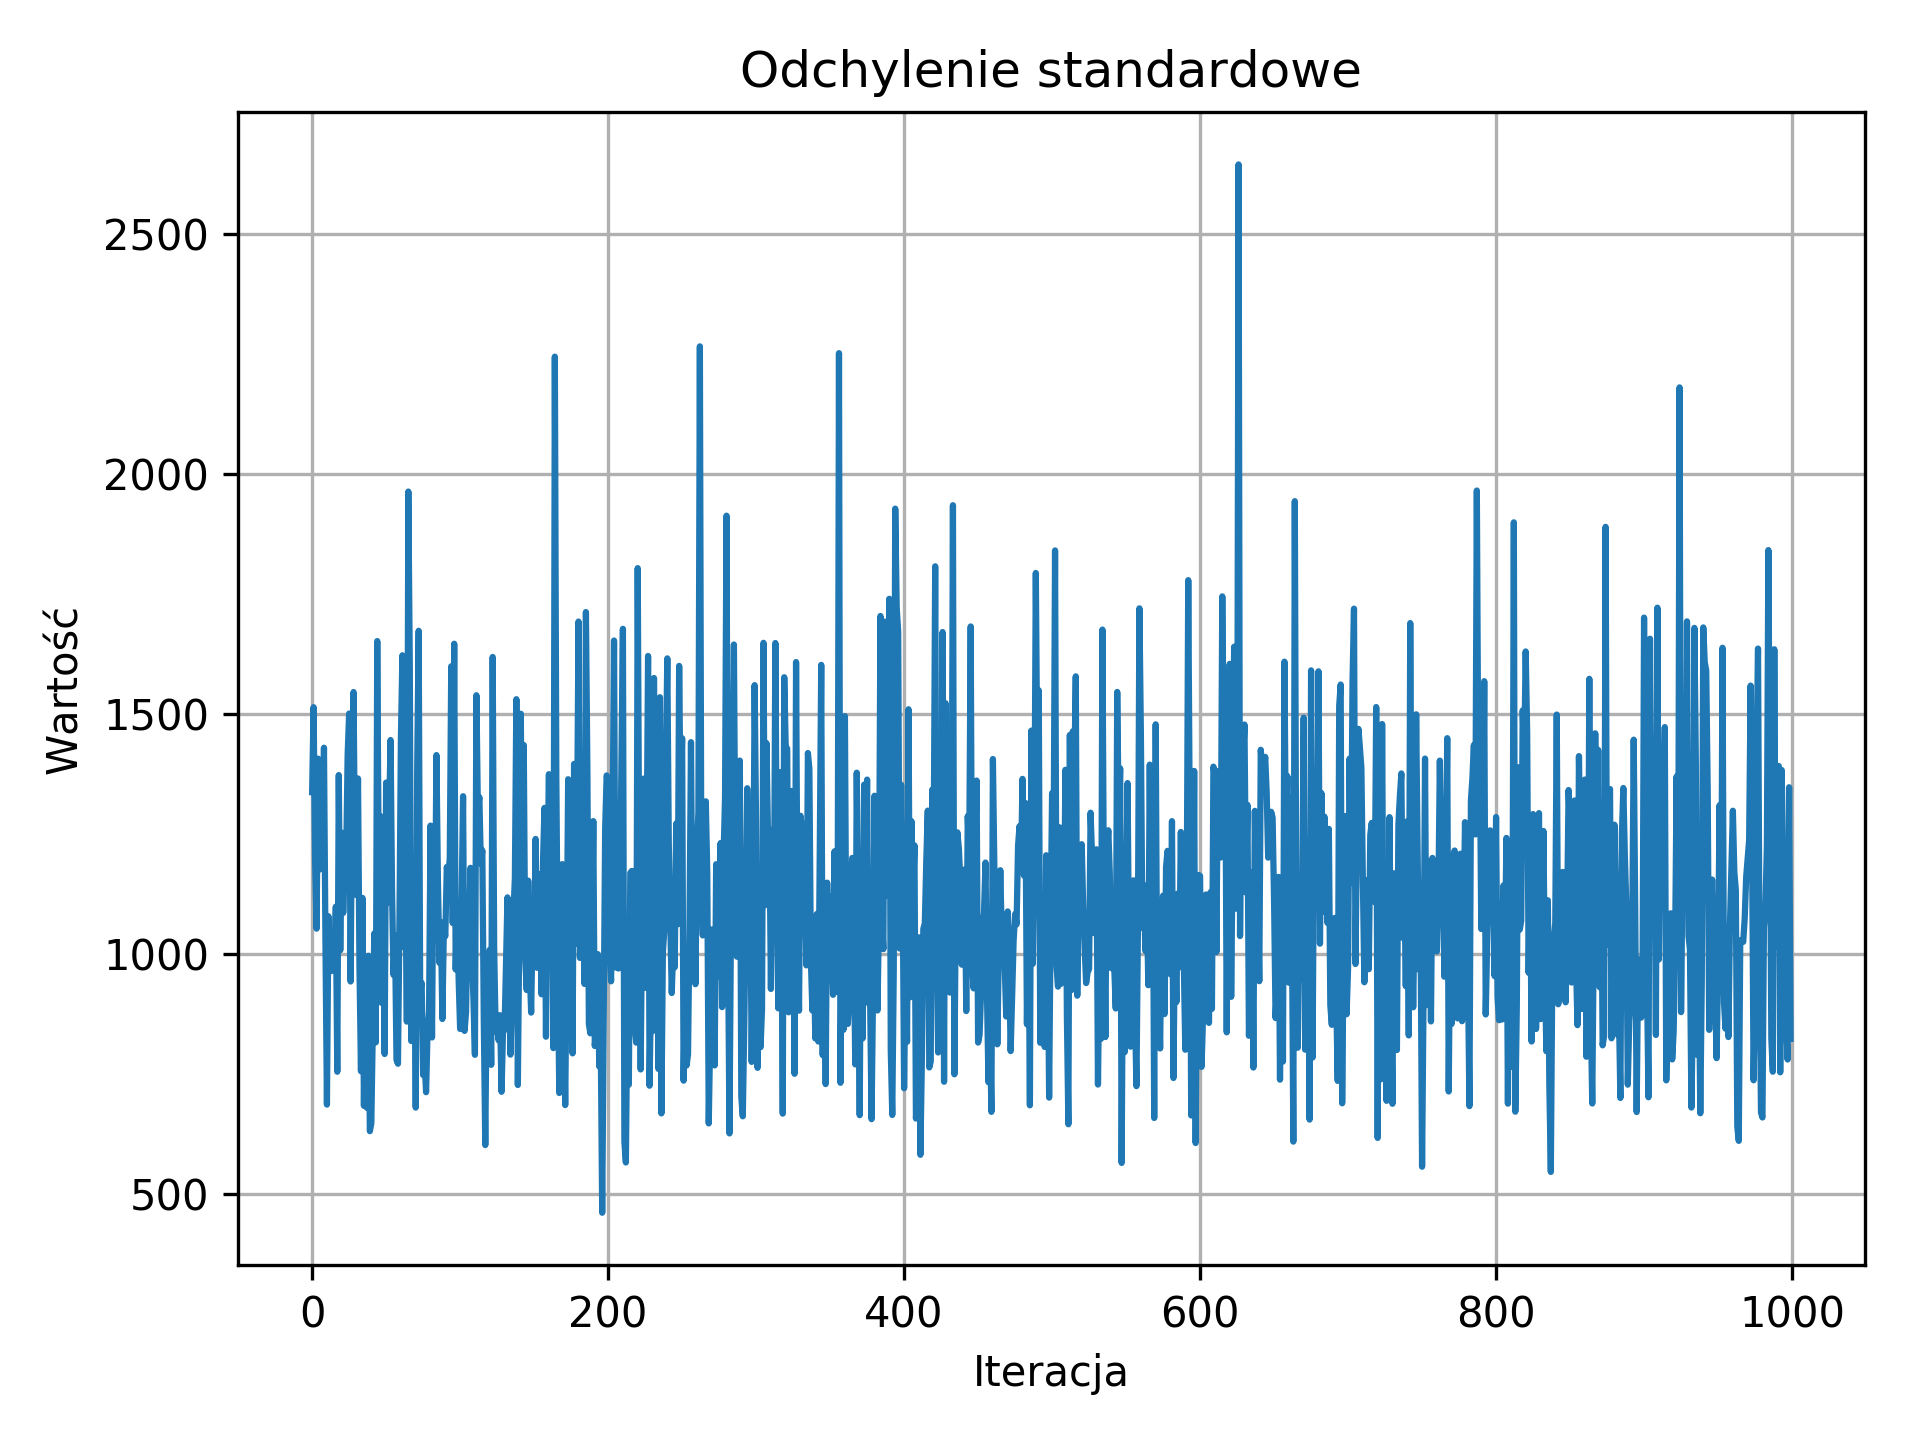
\includegraphics[width=0.55\textwidth]{threshold_1.png}
	\caption{Próg ustalony na 50 najlepszych kart.}
	\label{fig1}
\end{figure}


\begin{figure}[h]
	\centering					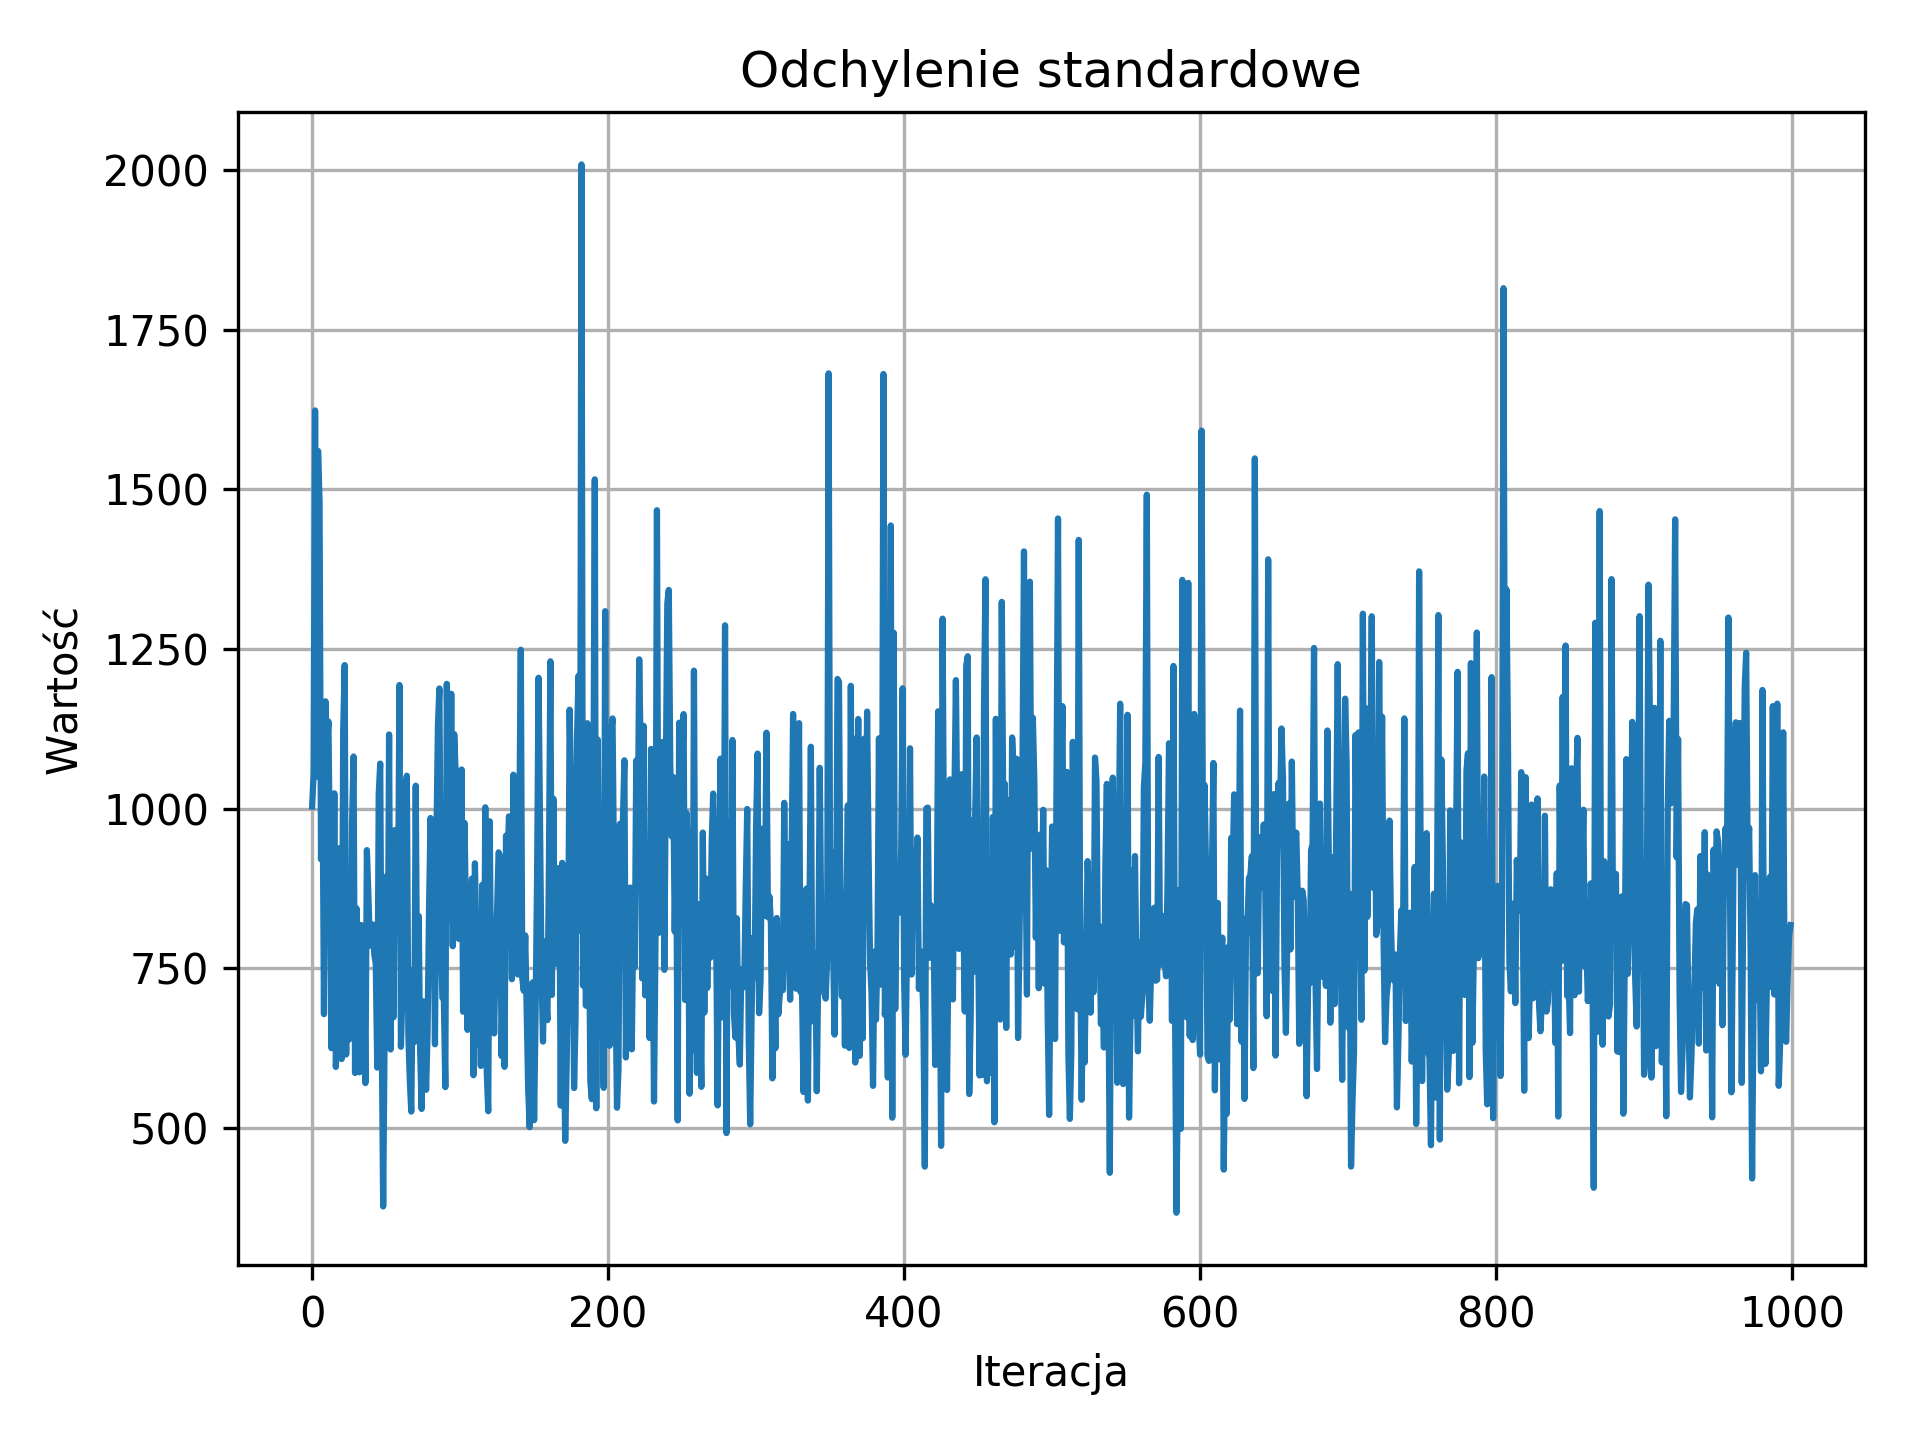
\includegraphics[width=0.55\textwidth]{threshold_2.png}
	\caption{Próg ustalony na 10 najlepszych kart.}
	\label{fig1}
\end{figure}

Powyższe wykresy pokazują różnice odchylenia standardowego w zależności od wybranego progu dla 100 kart. Są one zgodne z intuicją - dla większej wartości progu odchylenie standardowe wykazuje większe wahania. 

\newpage

\subsection{Selekcja proporcjonalna}


\begin{figure}[ht]
	\centering					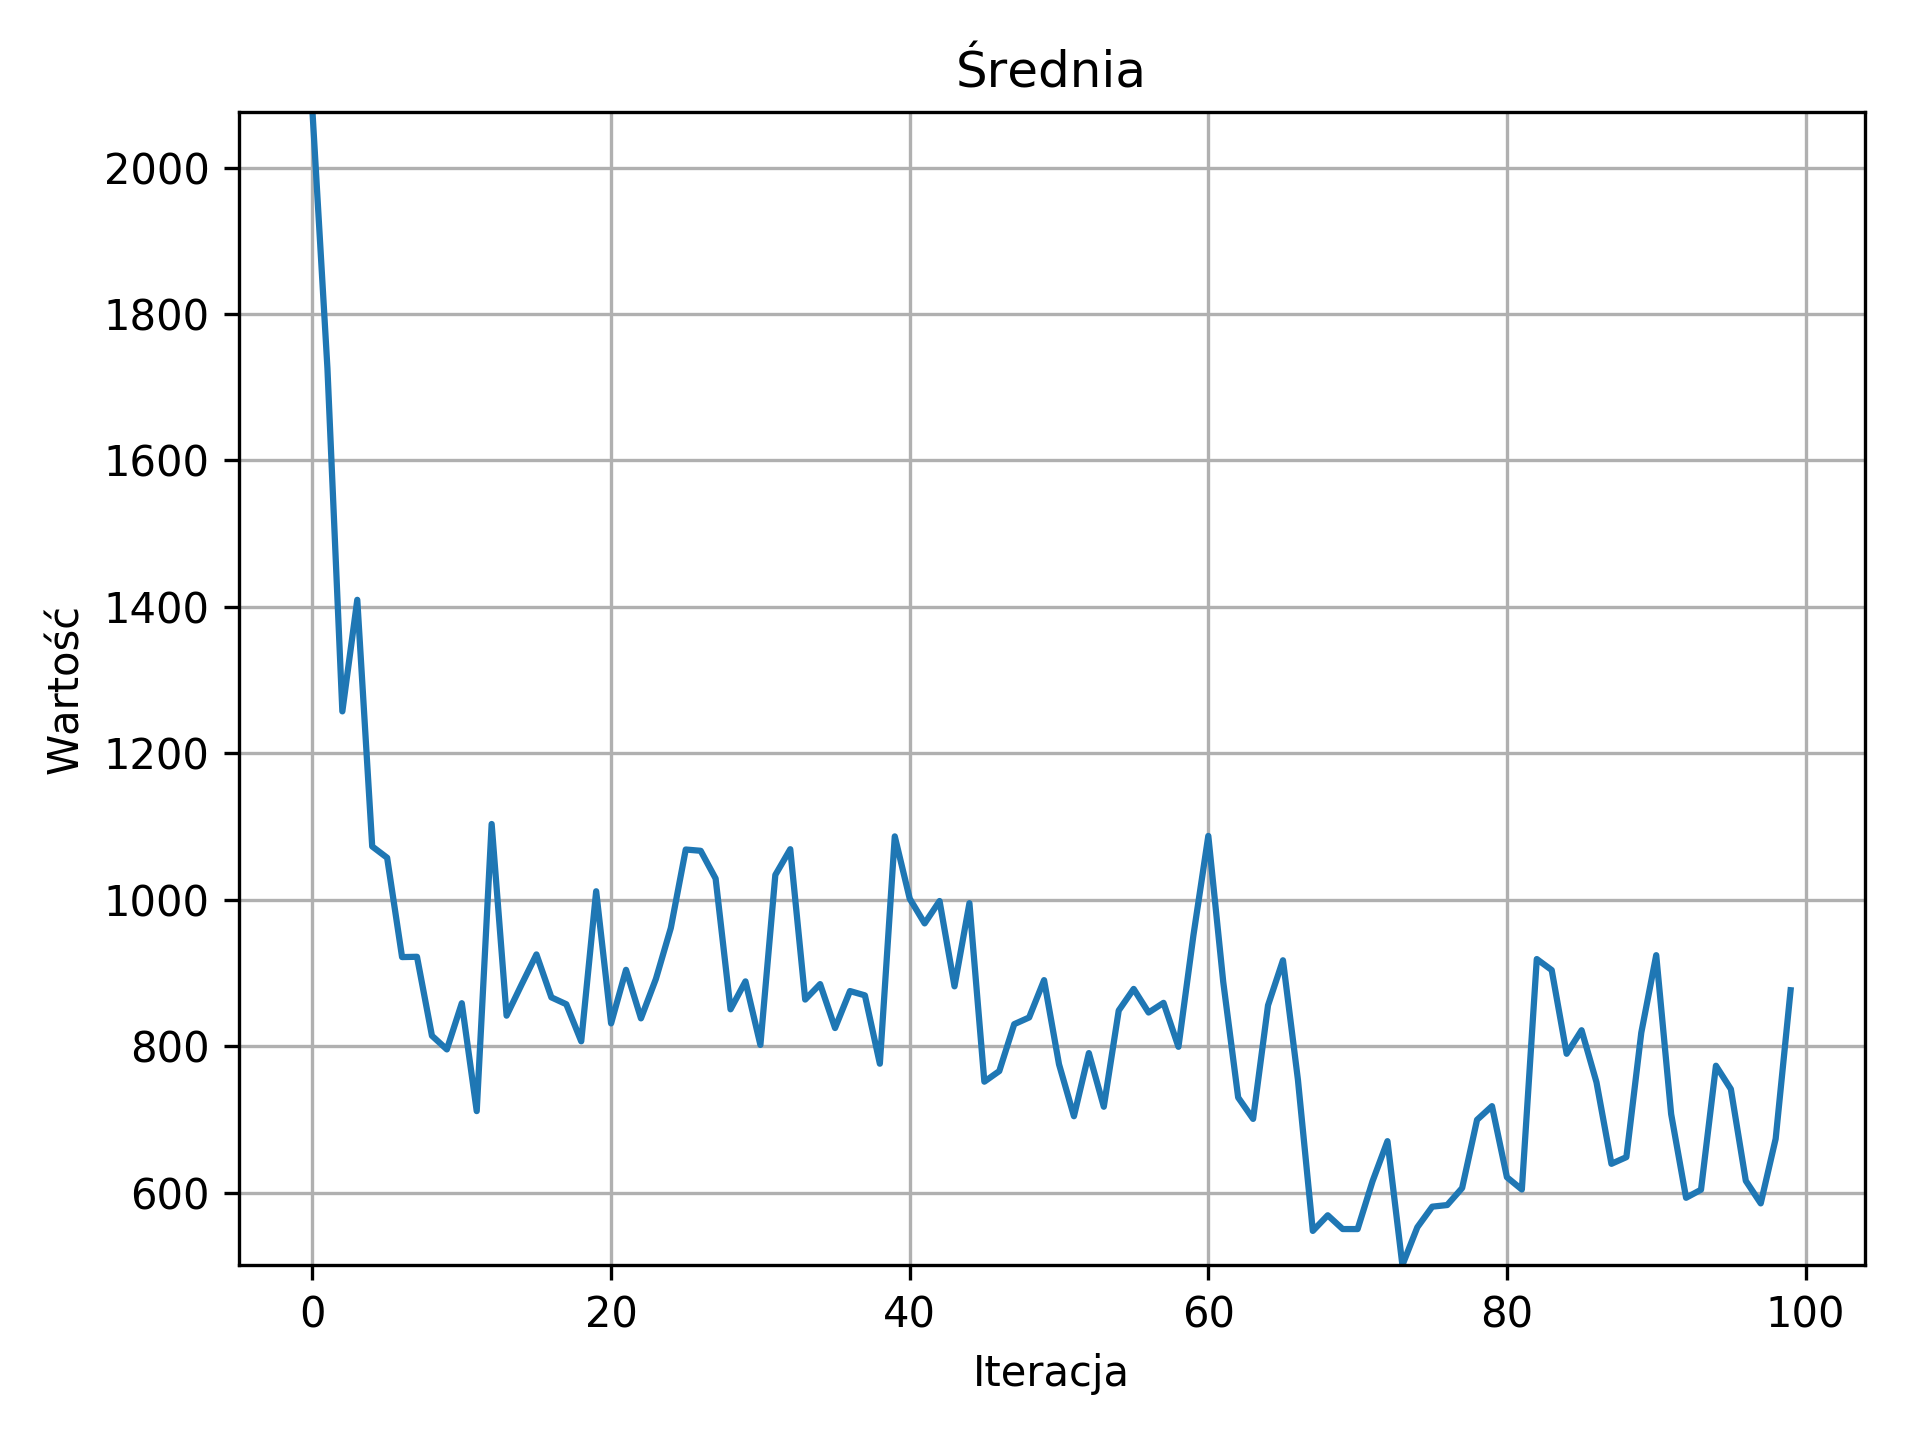
\includegraphics[width=0.55\textwidth]{roulette_1.png}
	\caption{Prawdopodobieństwo krzyżowania równe 0.1.}
	\label{fig1}
\end{figure}


\begin{figure}[ht]
	\centering					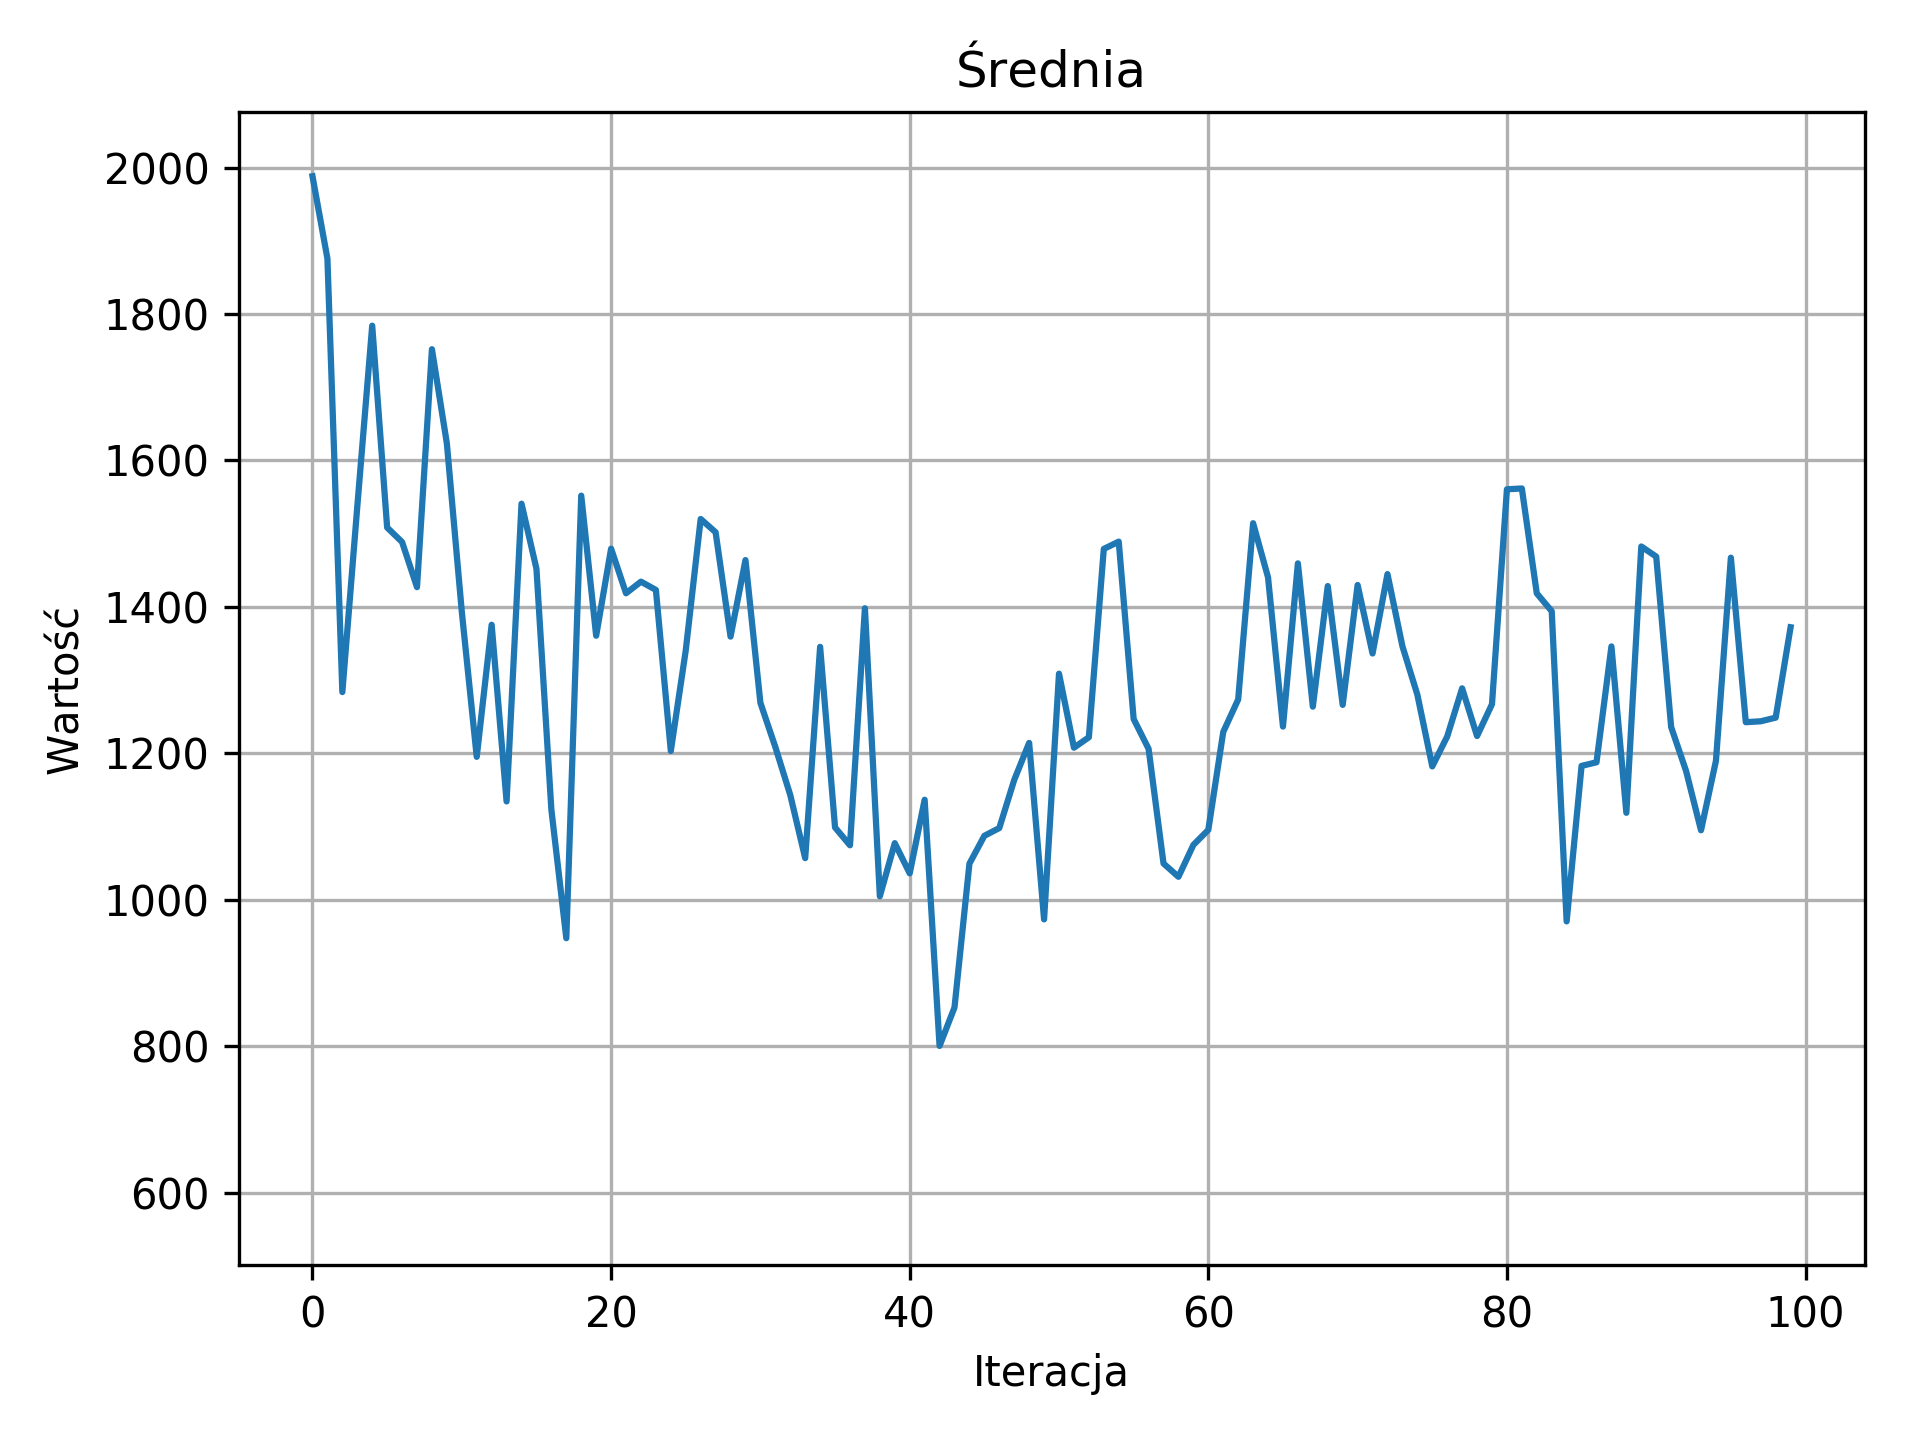
\includegraphics[width=0.55\textwidth]{roulette_2.png}
	\caption{Prawdopodobieństwo krzyżowania równe 0.5.}
	\label{fig1}
\end{figure}

Powyższe wykresy obrazują stopniowe zmniejszanie wartości średniej populacji. Przy małej wartości mutacji i krzyżowania proces ten dość szybko stabilizuje populacje(Rysunek 3). Natomiast dla dużego prawdopodobieństwa krzyżowania proces ten zachodzi wolniej z powodu krzyżowania lepszych osobników z gorszymi(Rysunek 4). 

\newpage

\begin{figure}[h]
	\centering					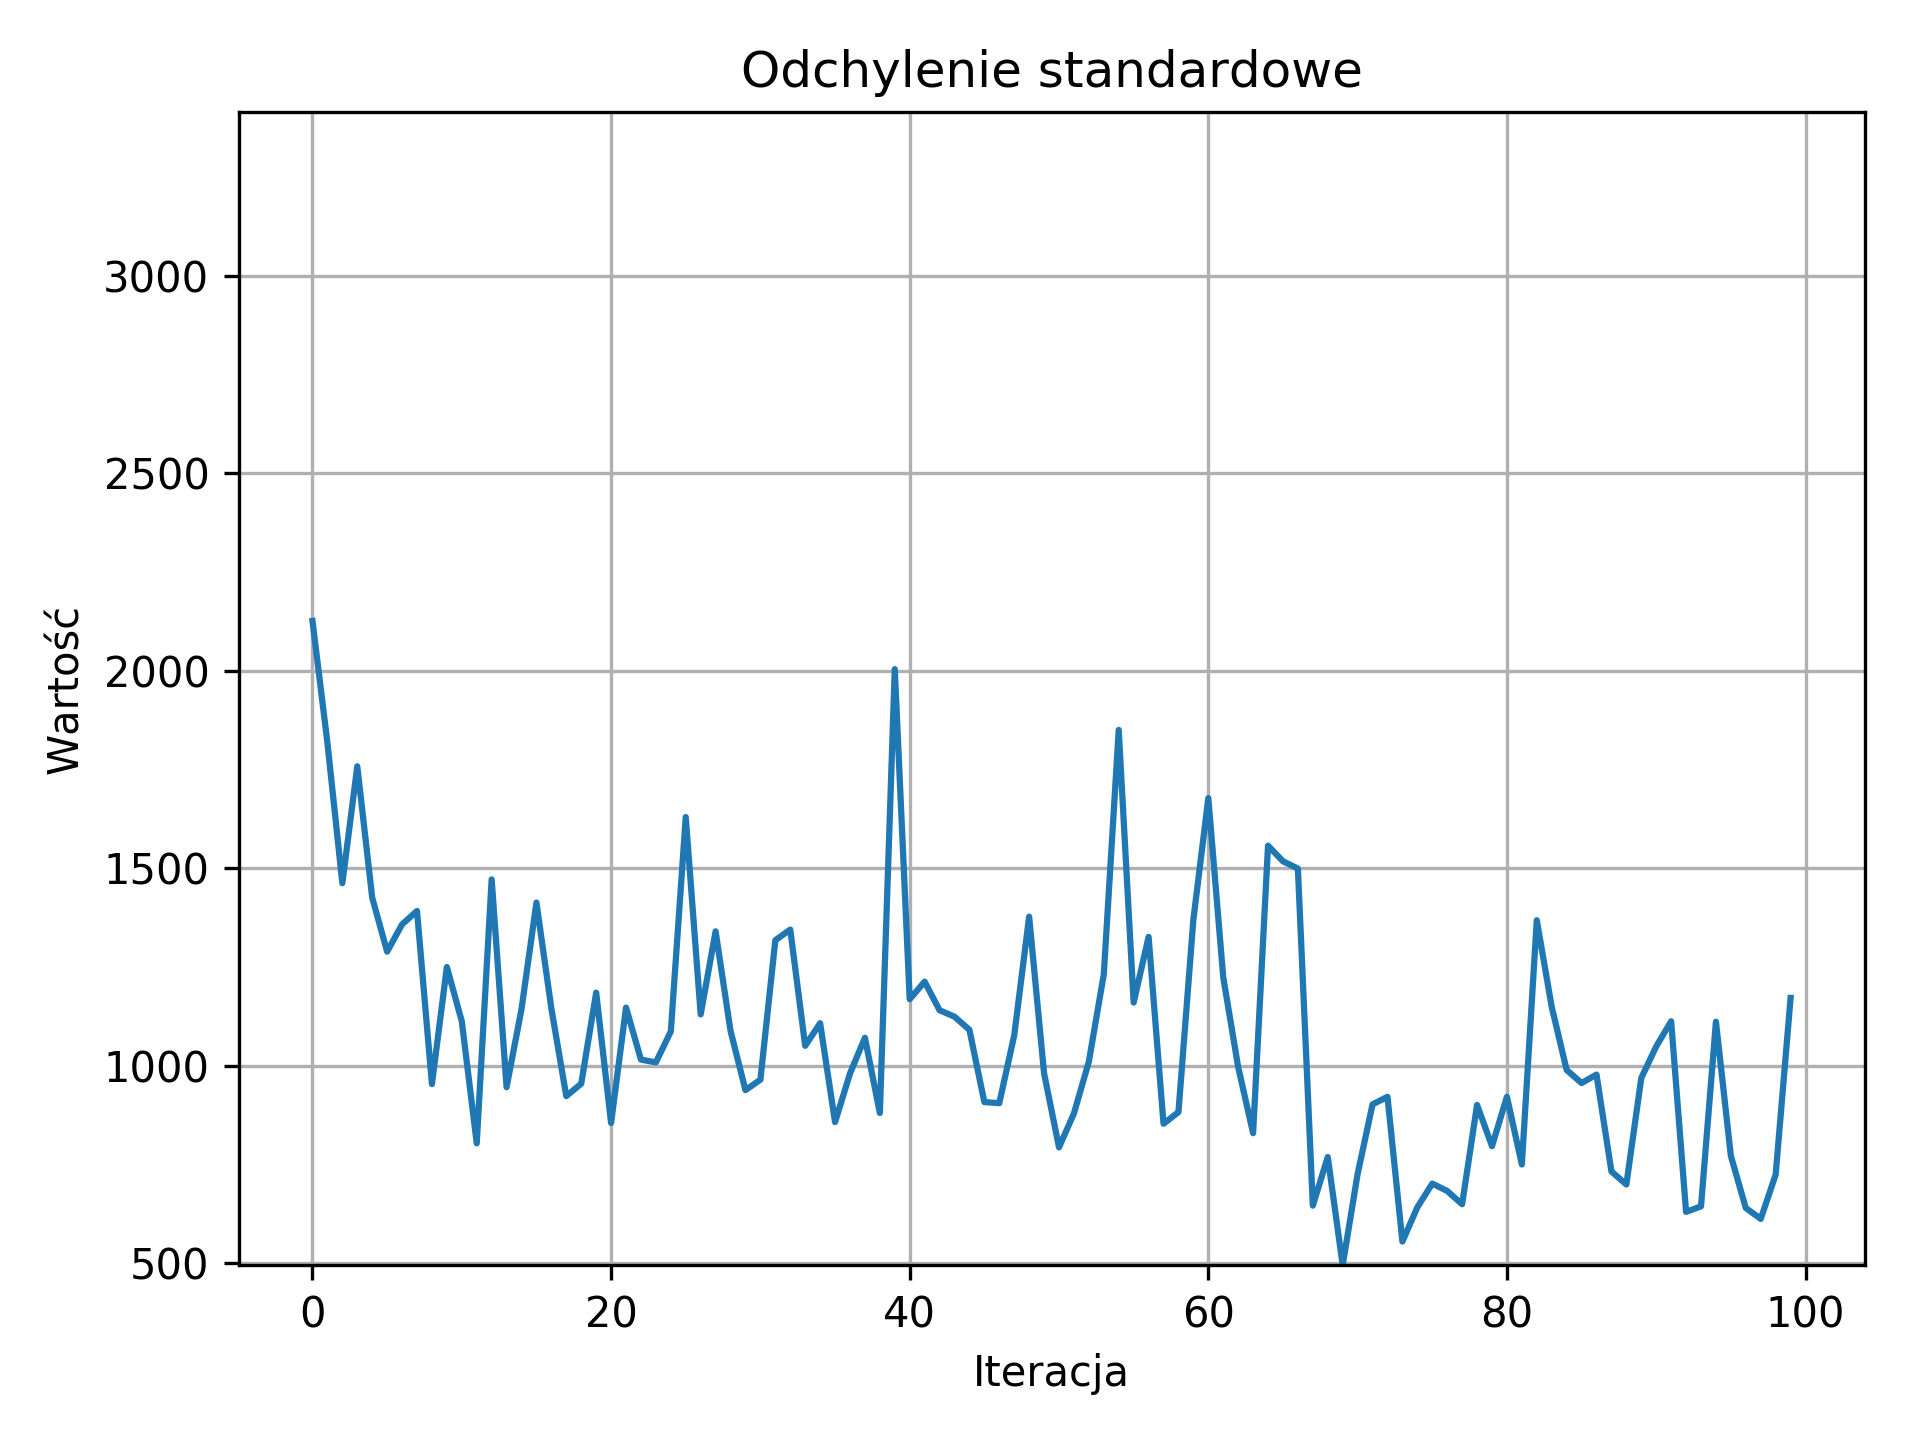
\includegraphics[width=0.55\textwidth]{roulette_3.png}
	\caption{Wartość \textit{beta} równa 1.}
	\label{fig1}
\end{figure}


\begin{figure}[h]
	\centering					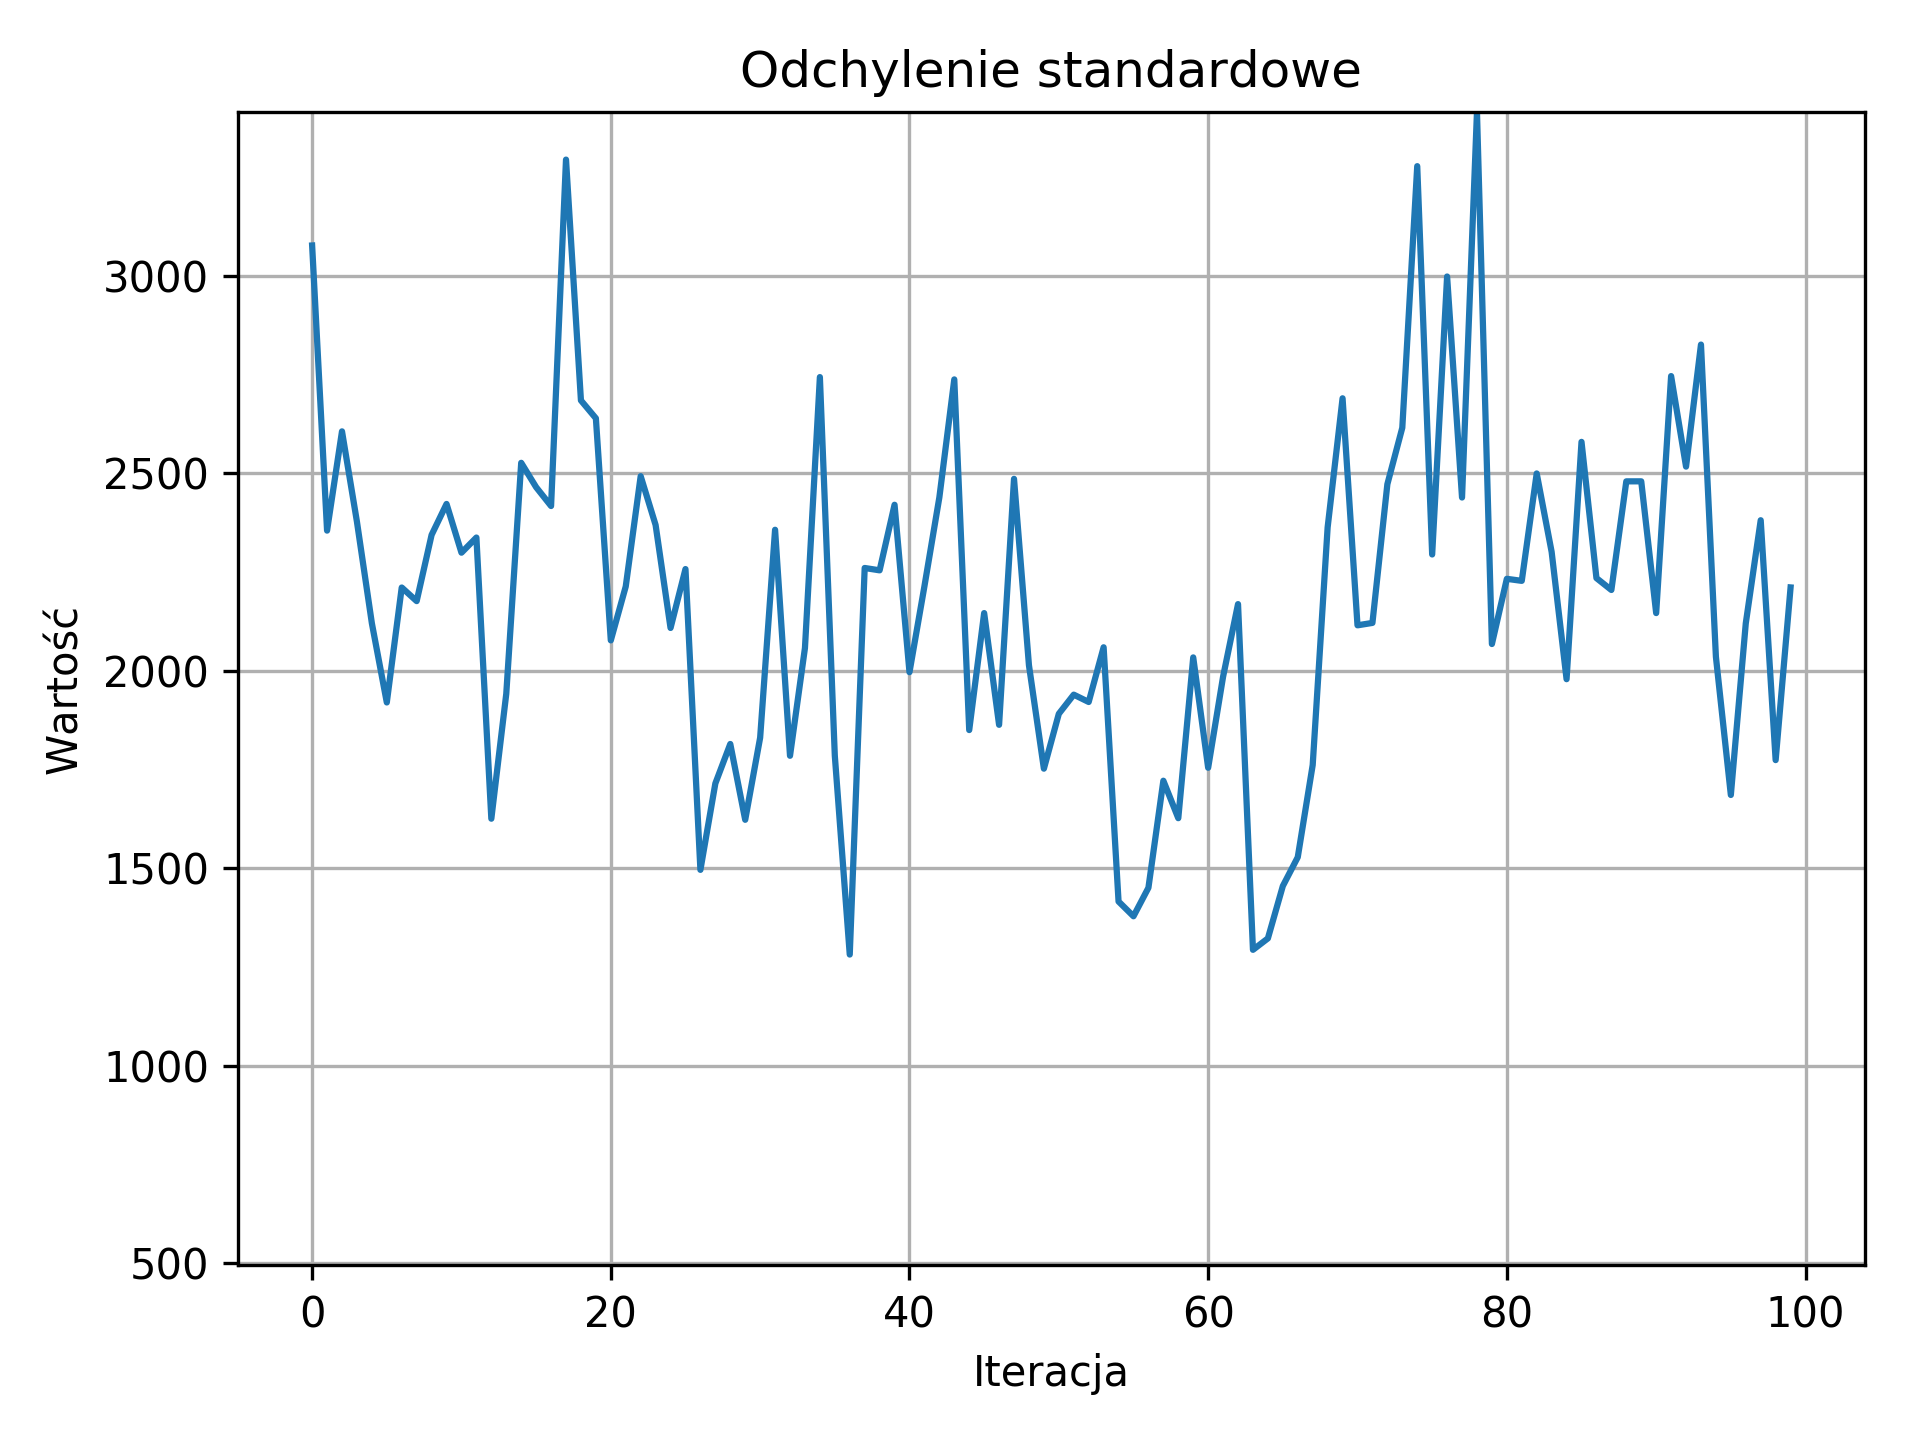
\includegraphics[width=0.55\textwidth]{roulette_4.png}
	\caption{Wartość \textit{beta} równa 0.5.}
	\label{fig1}
\end{figure}

Powyższe wykresy ukazują sposób wywierania presji przy selekcji proporcjonalnej przy obliczaniu wartości funkcji celu z użyciem wzoru  $exp(\frac{- \beta \cdot z_i}{z_{max}})$, gdzie $z_i$ odpowiada wartości celu $i$-tego osobnika. Im jest to większa wartość tym presja selekcji jest ostrzejsza - z tych powodów populacja z wykresu pierwszego ustabilizowała się szybciej i charakteryzuje się mniejszą wartością odchylenia standardowego.


\newpage

\subsection{Selekcja turniejowa}

\begin{figure}[h]
	\centering					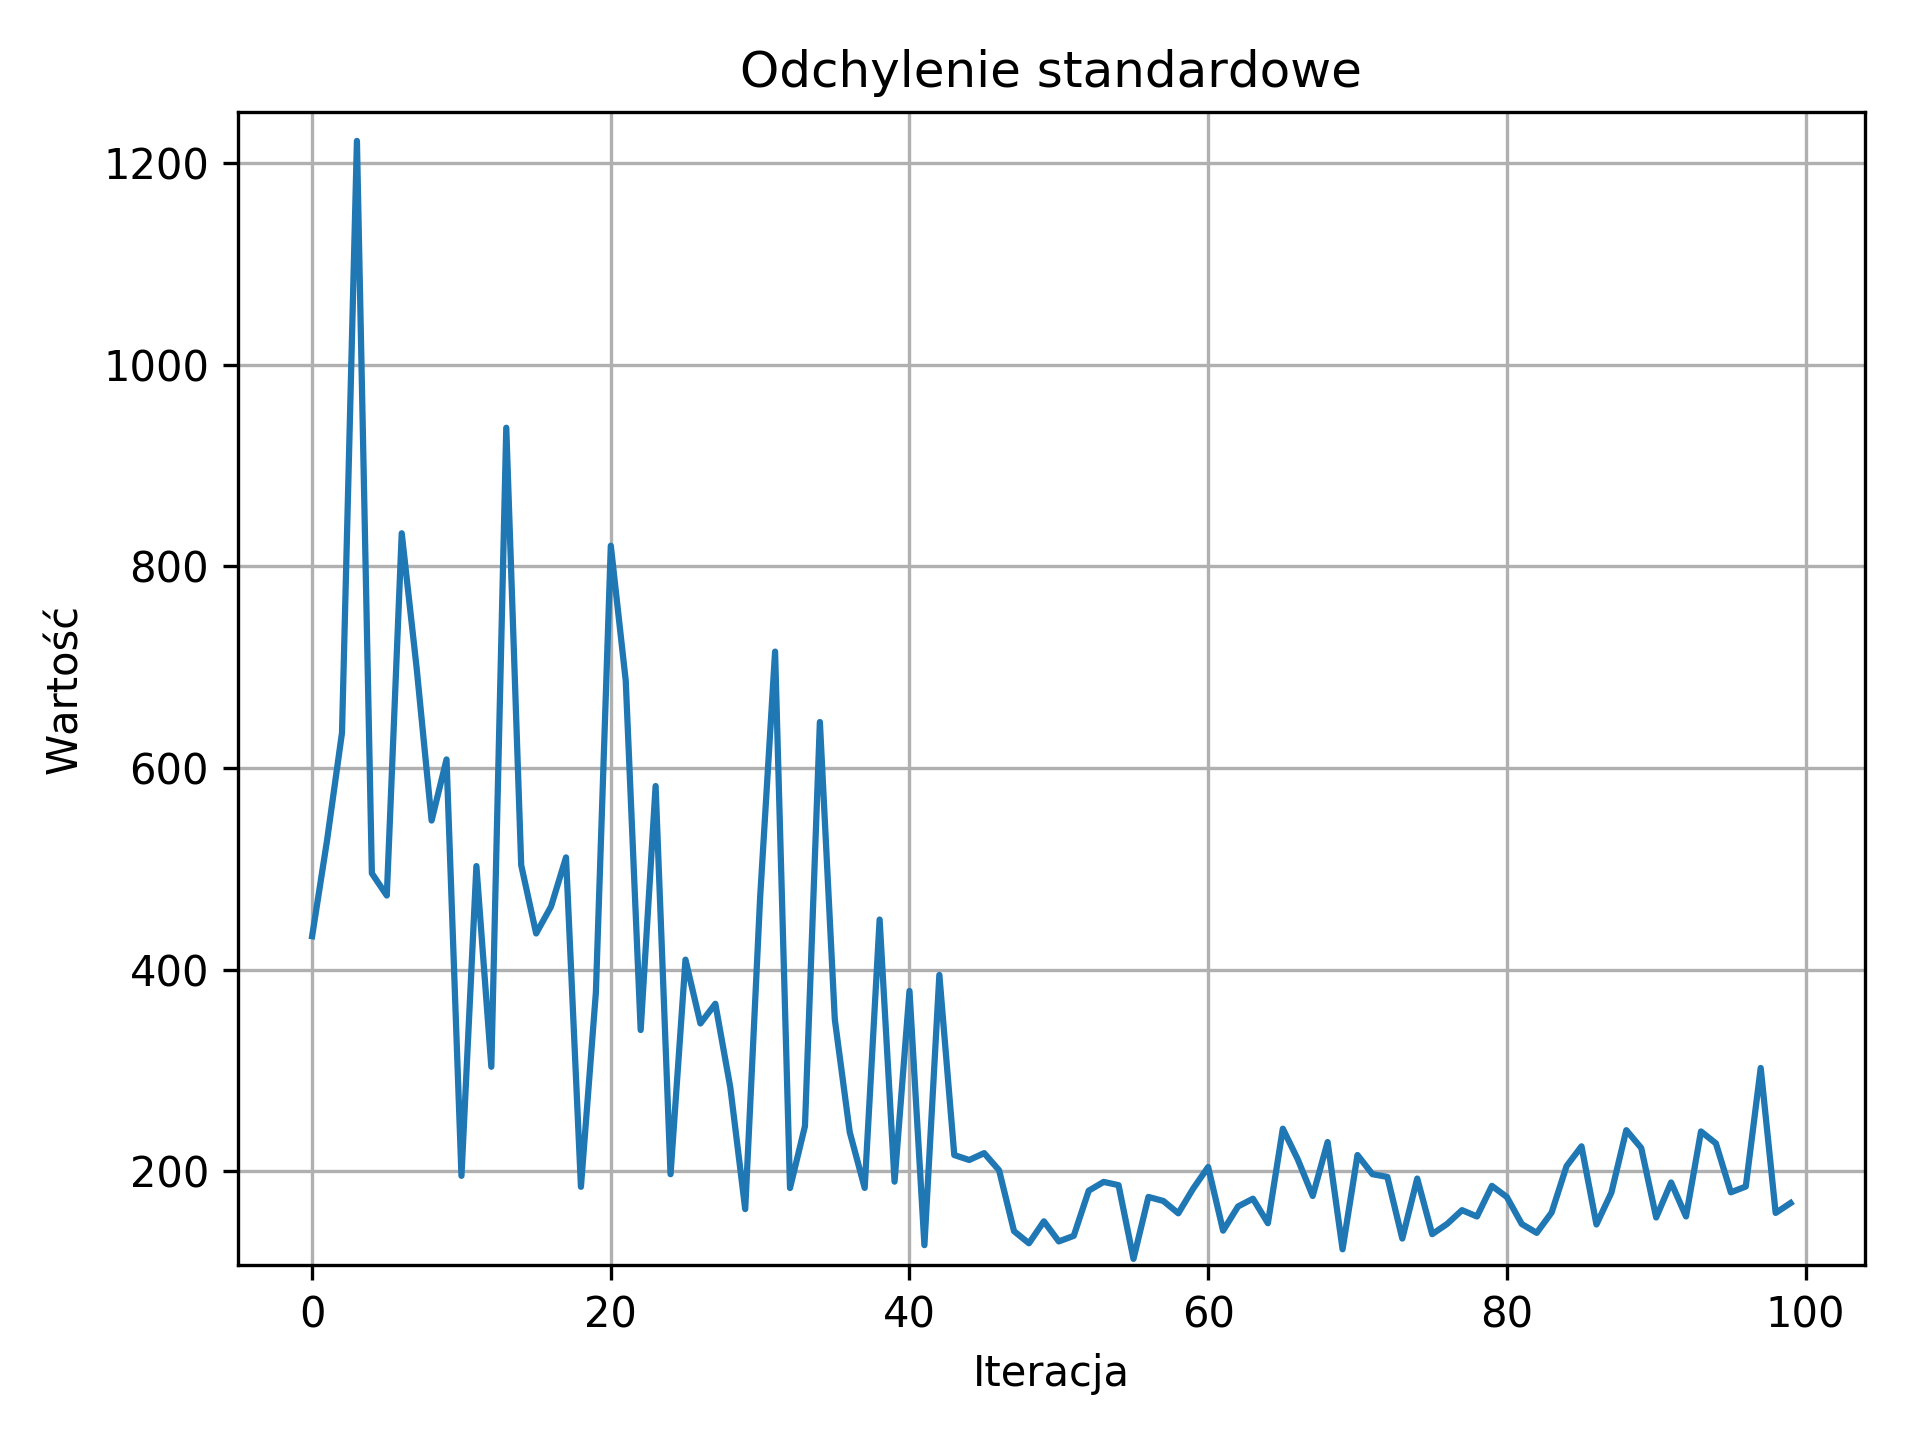
\includegraphics[width=0.55\textwidth]{tournament_1.png}
	\caption{Wartość szranków równa 50\% ilości kart.}
	\label{fig1}
\end{figure}


\begin{figure}[h]
	\centering					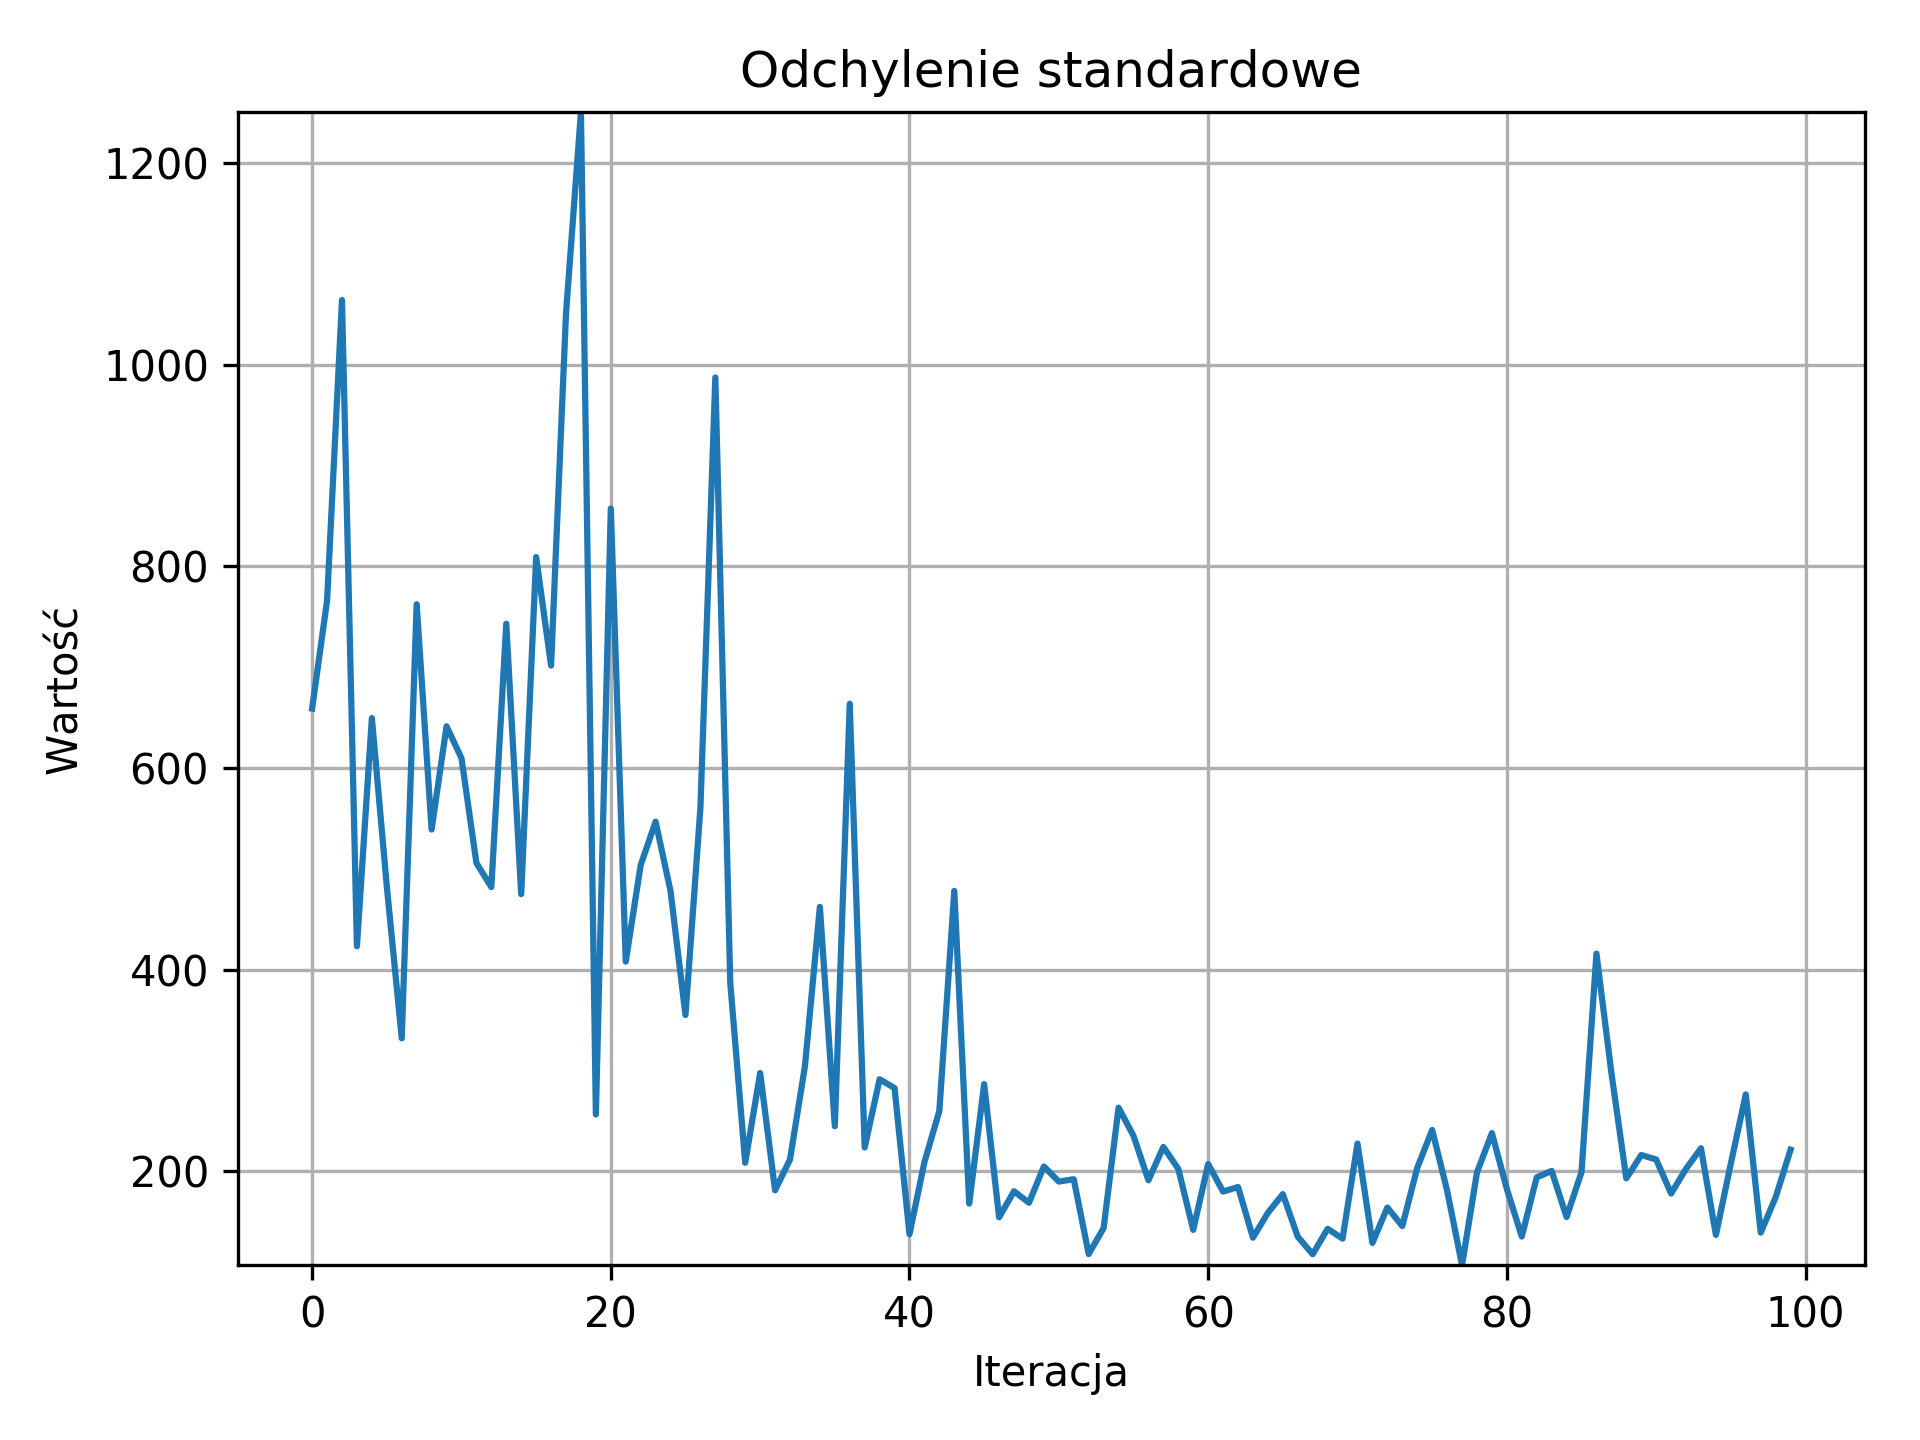
\includegraphics[width=0.55\textwidth]{tournament_2.png}
	\caption{Wartość szranków równa 10\% ilości kart.}
	\label{fig1}
\end{figure}

Powyższe wykresy ukazują wpływ wielkości szranków na stabilizacje populacji. Przy dużej wielkości szranków często wybierane są osobniki z czołówki populacji, stąd przy małej wartości mutacji populacji silnie zbiega do wartości najlepszego osobnika. W przypadku mniejszej wielkości szranków(Rysunek 8.) proces ten nie jest tak jednostajny. 

\newpage
\subsection{Badanie krzyżowania k-punktowego}
\begin{figure}[h]
	\centering					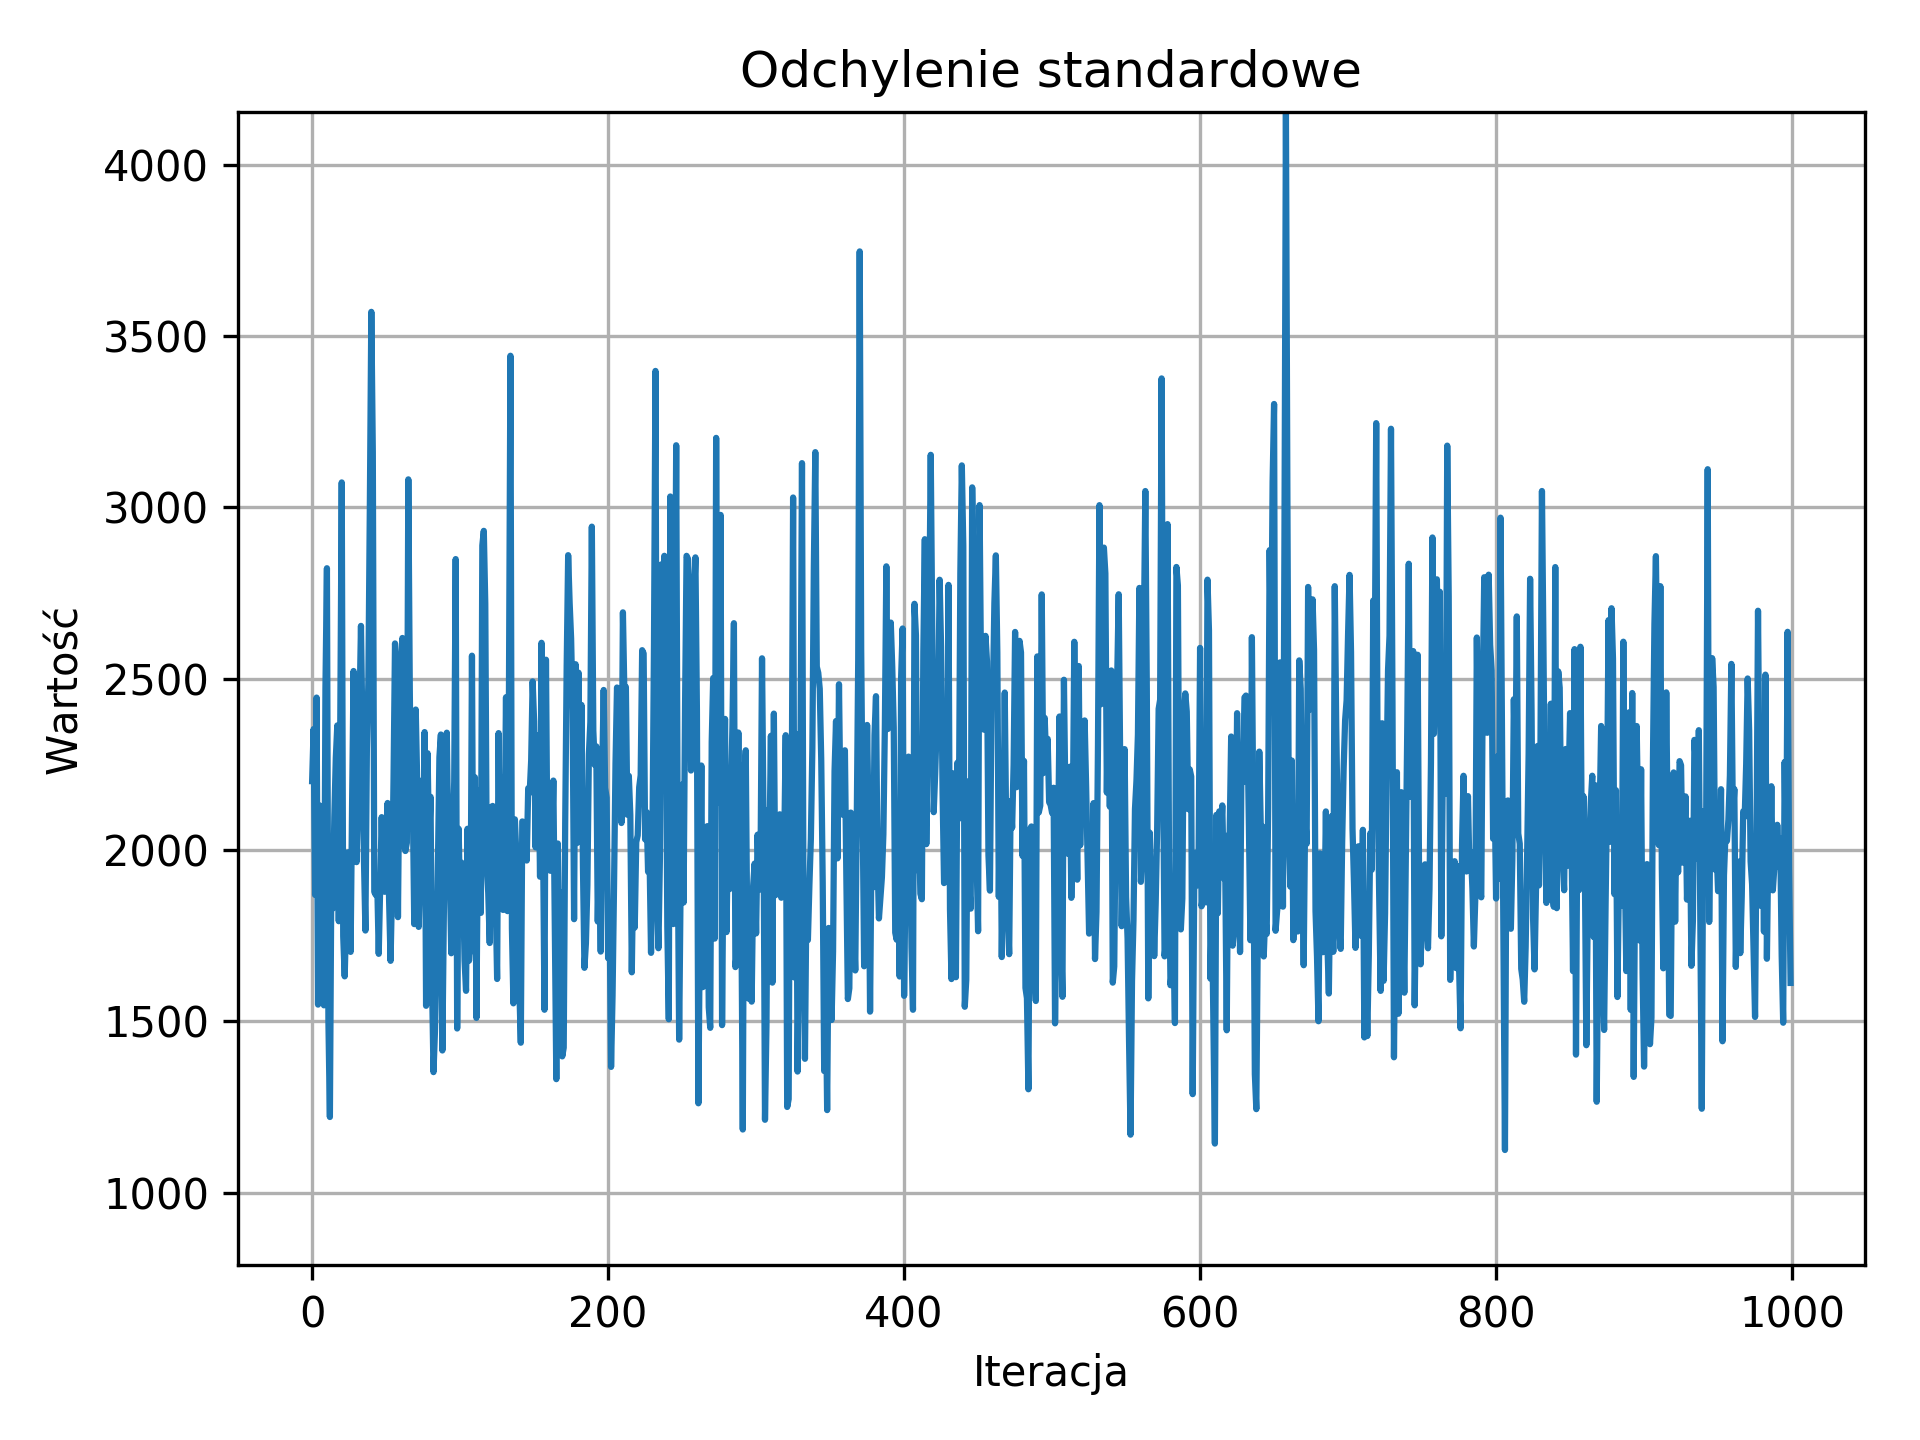
\includegraphics[width=0.55\textwidth]{k_1.png}
	\caption{Przebieg dla krzyżowania z wyborem właściciela karty dla każdej osobno.}
	\label{fig1}
\end{figure}


\begin{figure}[h]
	\centering					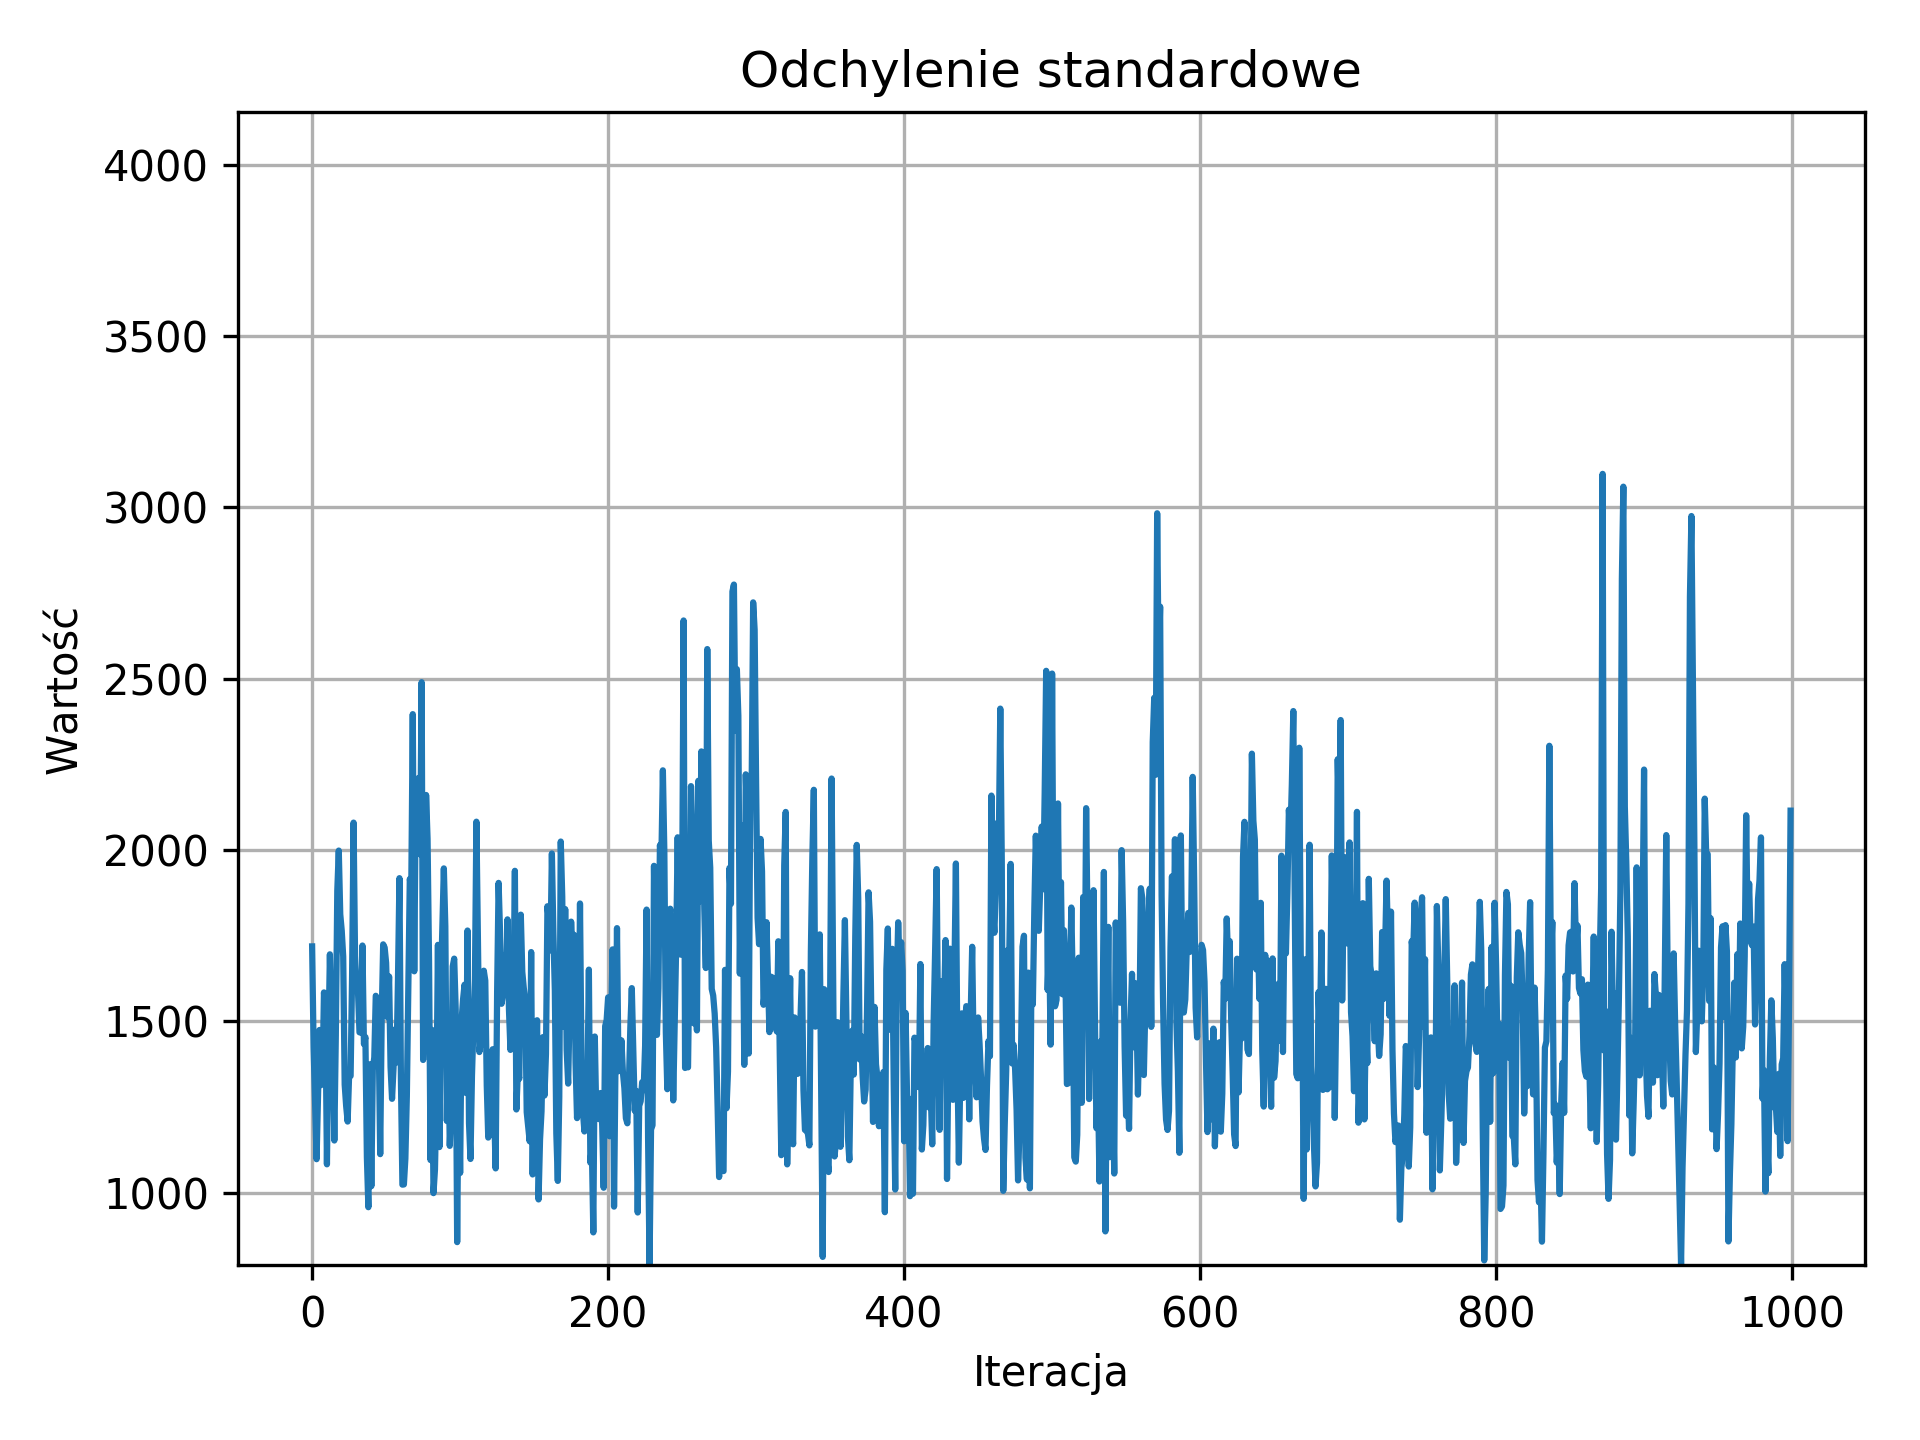
\includegraphics[width=0.55\textwidth]{k_2.png}
	\caption{Przebieg dla krzyżowania k-punktowego, k = 5.}
	\label{fig1}
\end{figure}

Jak można wywnioskować z wykresów krzyżowanie k-punktowe nie wpływa tak znacząco na poszerzanie przestrzeni przeszukiwań algorytmu jak wybór właściciela dla każego osobnika z osoba i jest to zgodne z przewidywaniami. Testy były przeprowadzone dla osobnika reprezentowanego przez 100 kart. 

\newpage
\subsection{Rozmiar populacji}
\begin{figure}[h]
	\centering					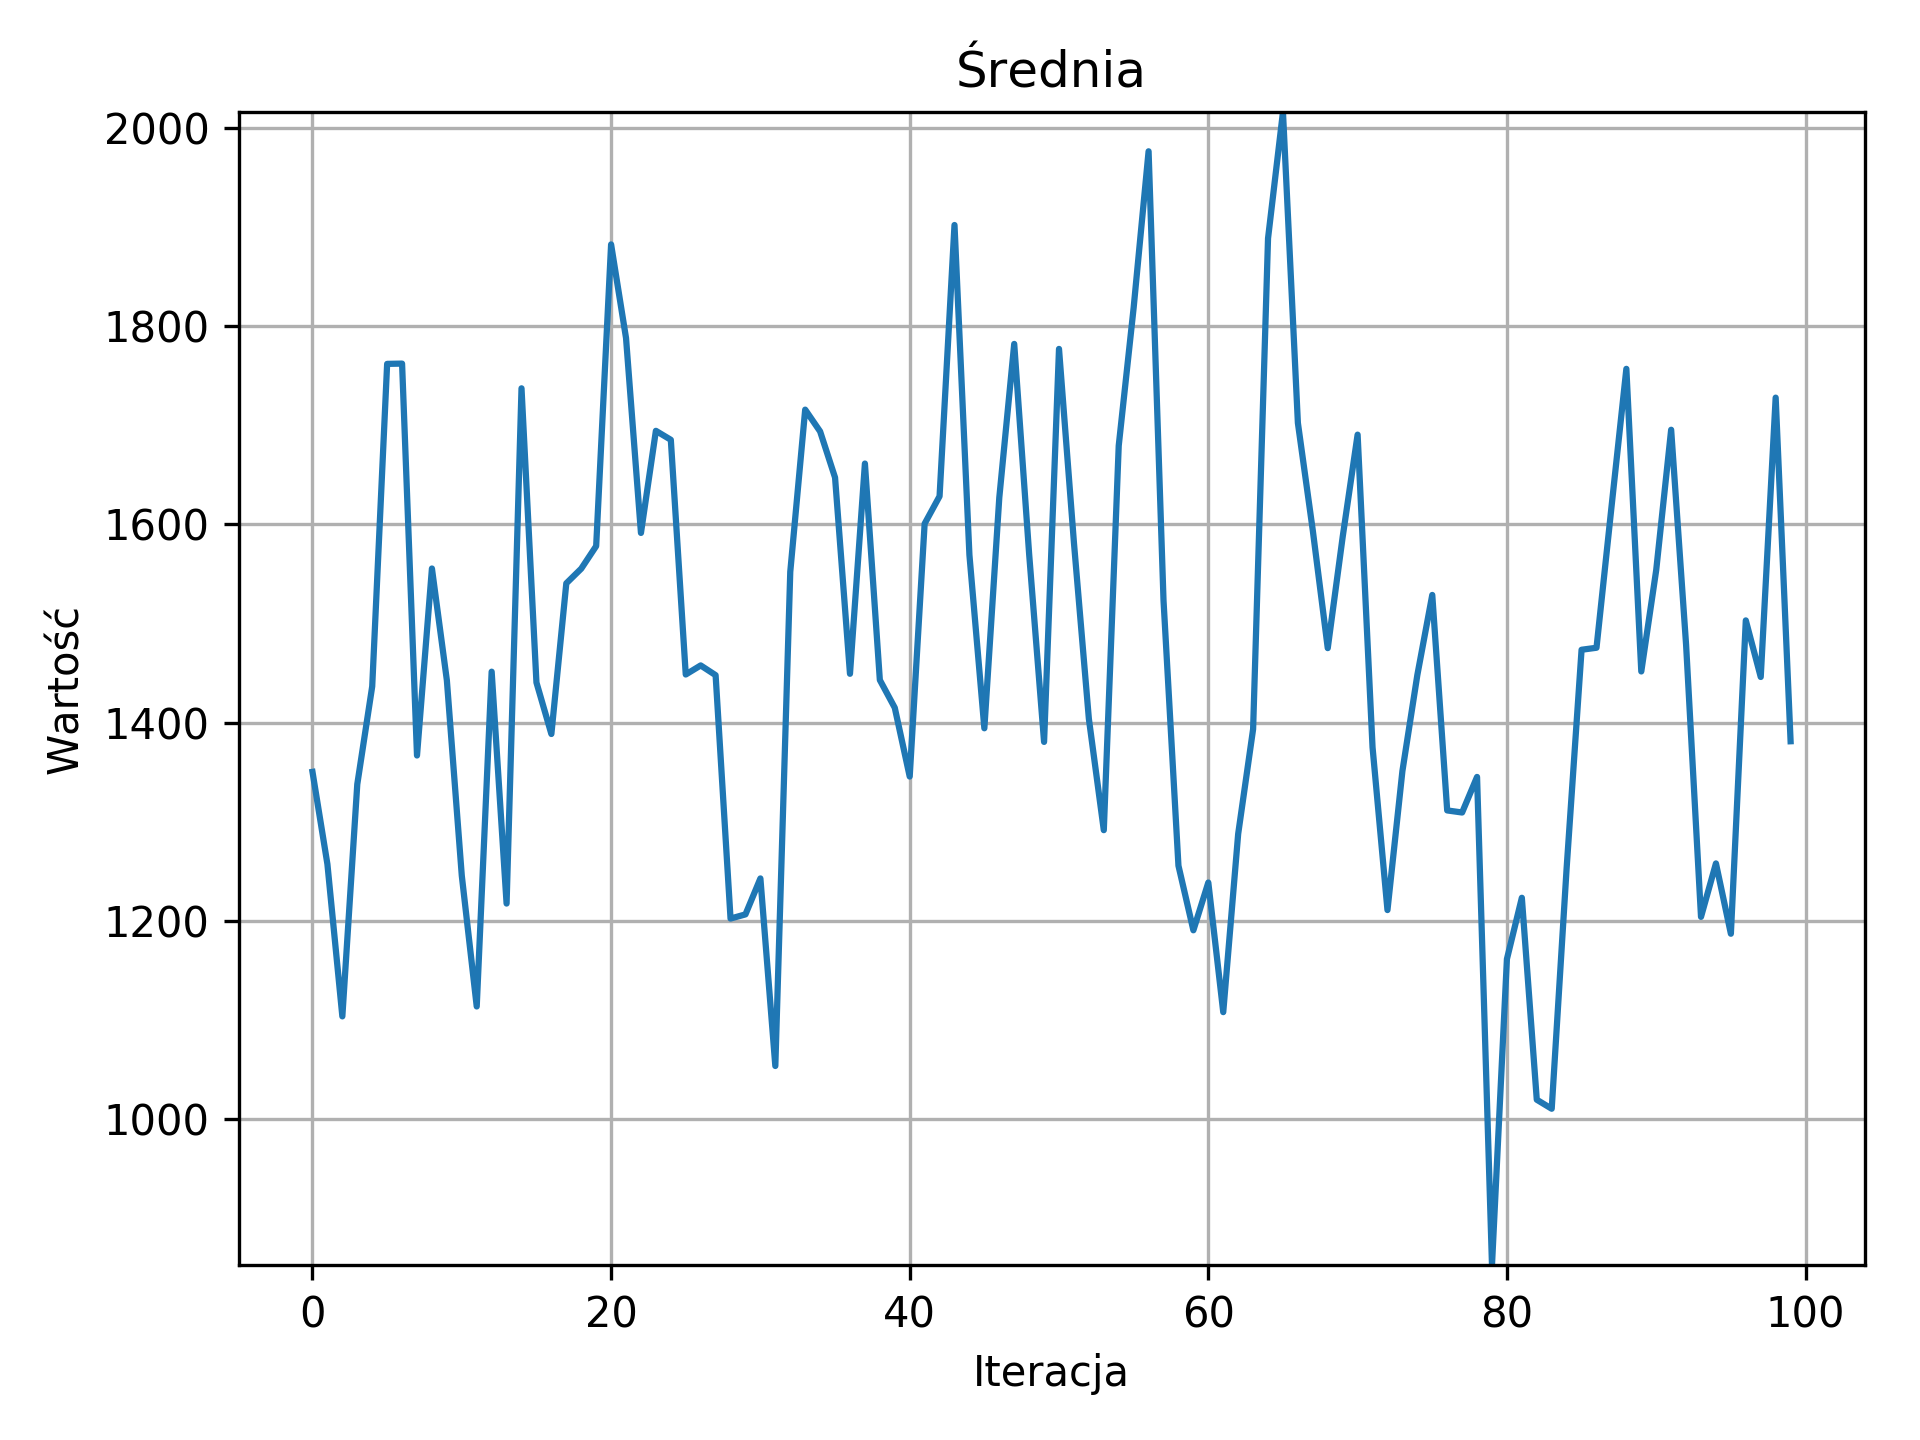
\includegraphics[width=0.55\textwidth]{pop_1.png}
	\caption{Rozmiar populacji równy 100.}
	\label{fig1}
\end{figure}


\begin{figure}[h]
	\centering					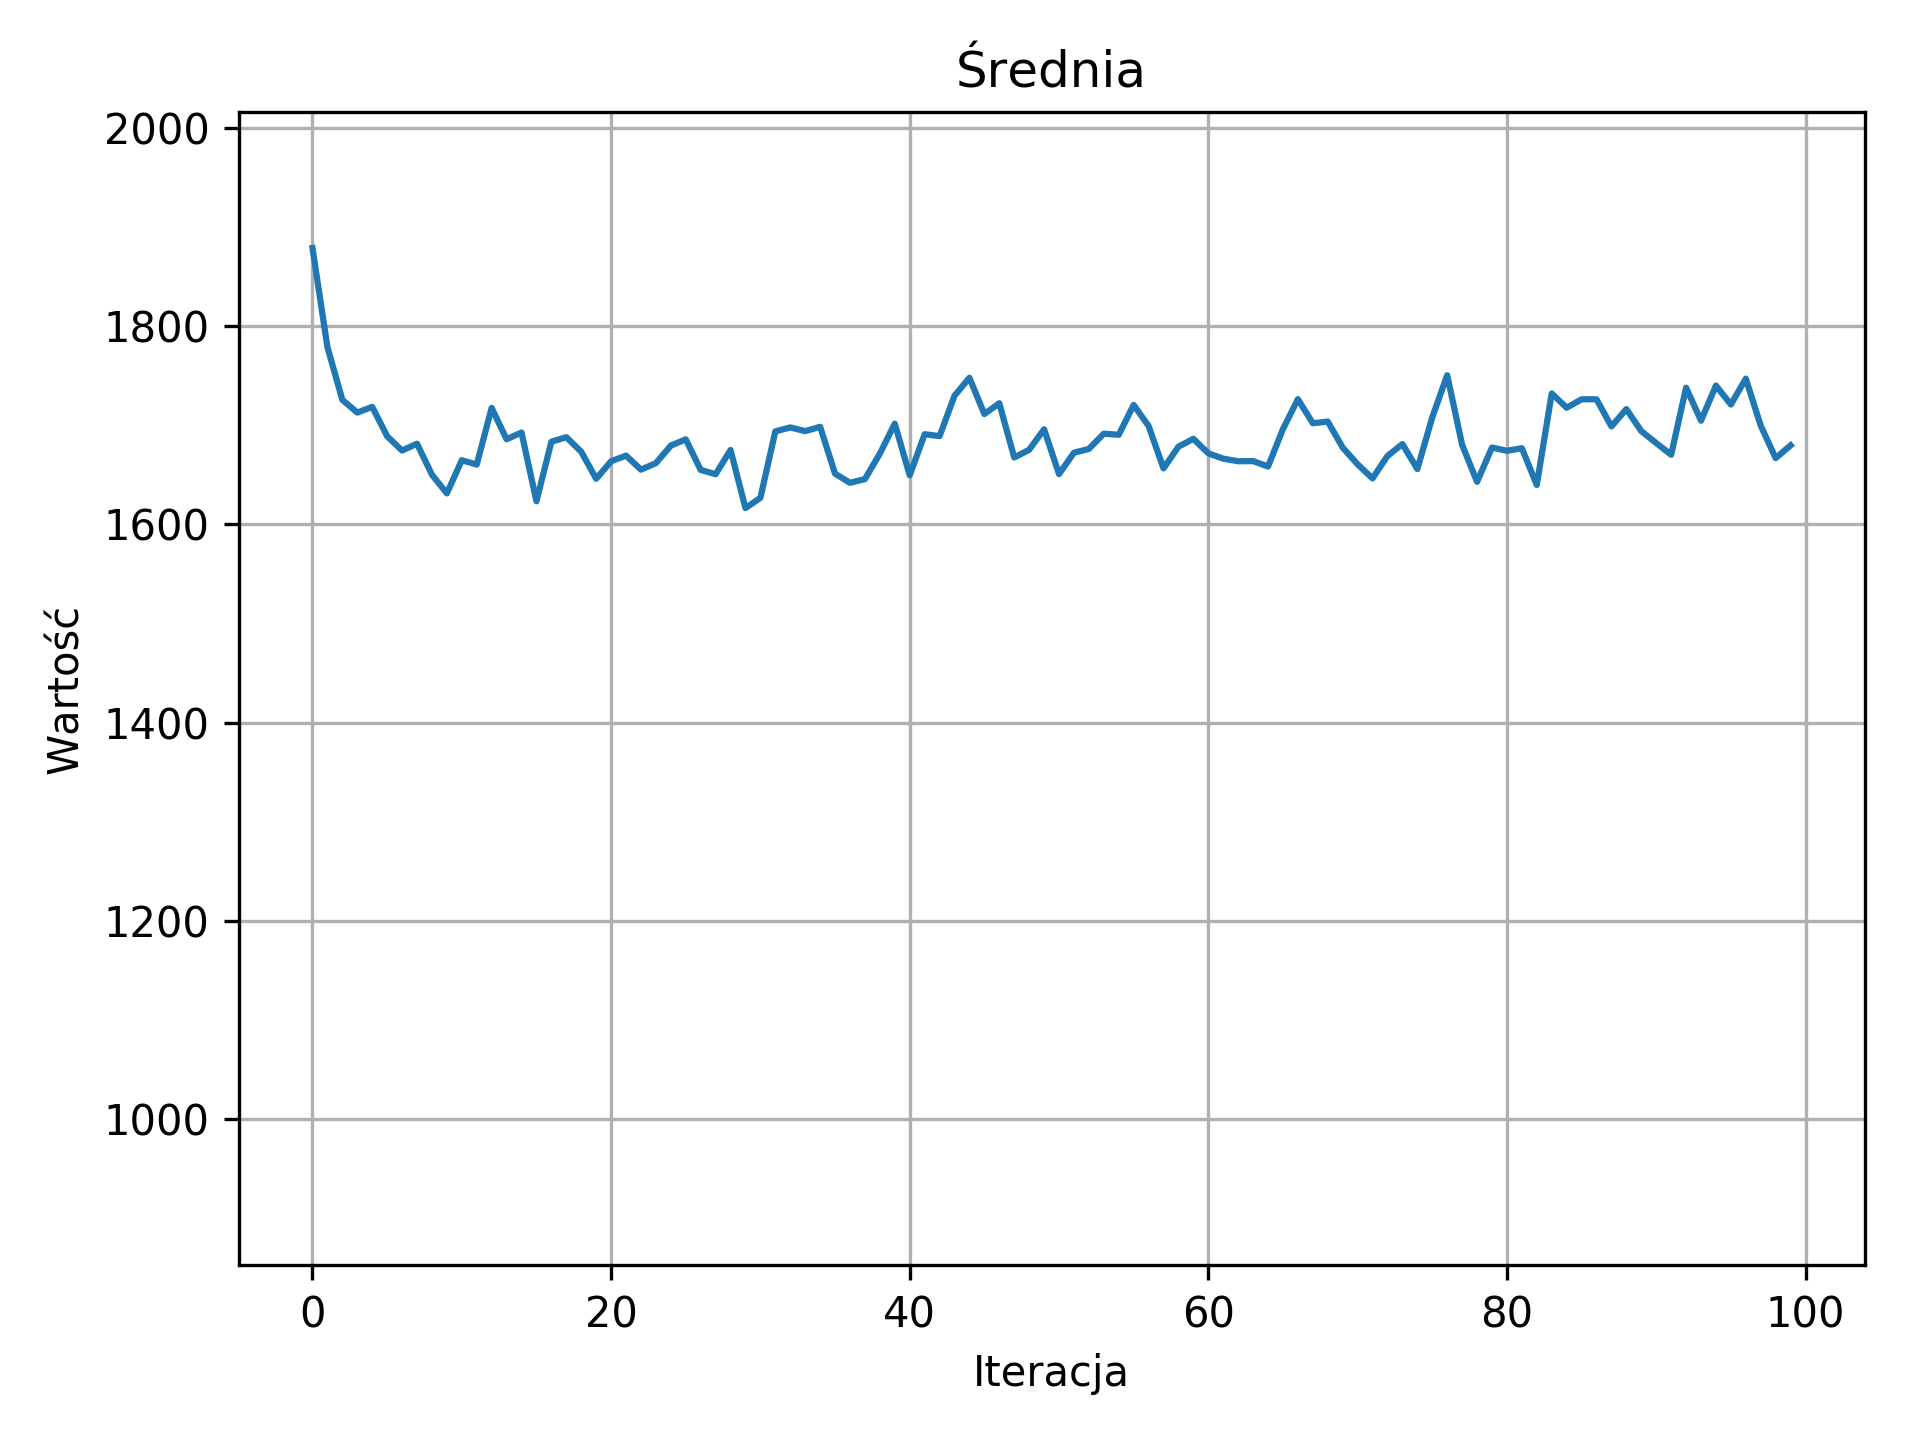
\includegraphics[width=0.55\textwidth]{pop_2.png}
	\caption{Rozmiar populacji równy 10000.}
	\label{fig1}
\end{figure}

Przy badaniach została wykorzystana selekcja proporcjonalna z wartością \textit{beta} równą 1 i prawdopodobieństwem krzyżowania równym 0.3. Duża populacja nie może zostać zaburzona w tak prosty sposób i oscyluje ona niezmiennie wokół jednej wartości.   

\subsection{Komentarz do wyników}

Przedstawione wykresy pokazują działanie zaimplementowanych algorytmów. Populacja zachowuje się zgodnie z oczekiwaniami - wraz z iteracjami zmniejsza się wartość odchylenia standardowego i średniej. Problemem okazała się za to przestrzeń przy zbliżonych wartościach oczekiwanych dla obu stosów.

Niepokojące były wykresy przedstawiające wartość fukncji celu najepszego elementu populacji. Wyglądały one następująco:
\begin{figure}[H]
	\centering					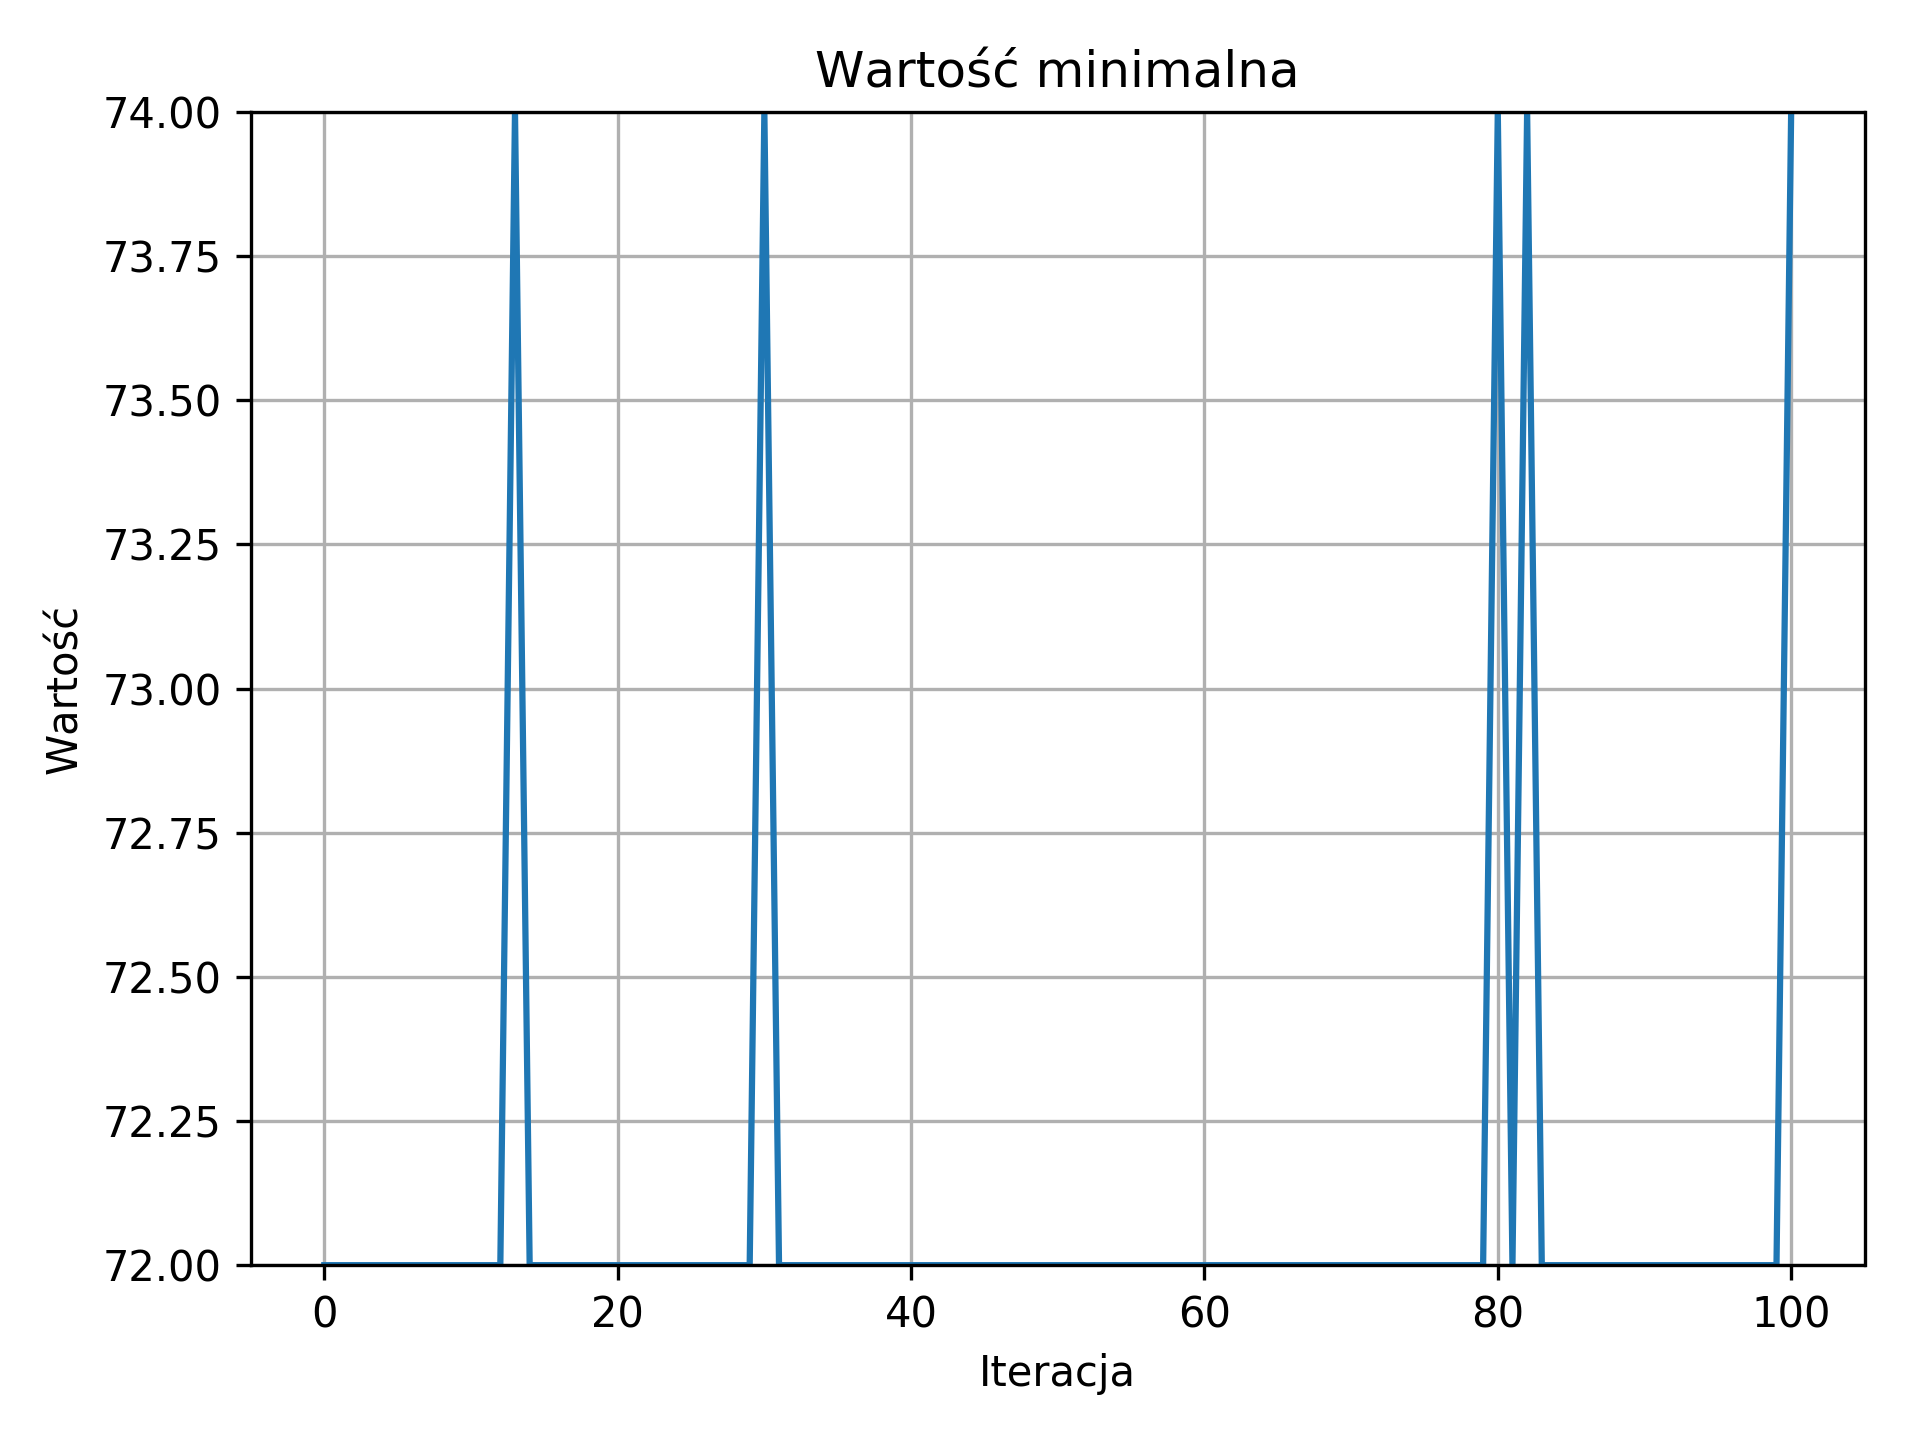
\includegraphics[width=0.55\textwidth]{two_group.png}
	\caption{Minimlna wartość funkcji celu w zależności od numeru iteracji.}
	\label{fig1}
\end{figure}

Na wykresie tym widać, że najlepsza znaleziona wartość funkcji celu znajdowała się już w populacji początkowej. Tylko nieliczne populacje nie zawierały elementu optymalnego. Jednocześnie, jak pokazują inne statystyki, takie jak średnia wartość funkcji celu czy odchylenie standardowe, populacja w tym czasie zmieniała się znacznie. Wzbudziło to tak duże wątpliwości, że zdecydowano się na dokładniejsze zbadanie przeszukiwanej przestrzeni.

Badania przestrzeni realizowano poprzez przejście po całej przestrzeni i zapisanie poszczególnych uzyskanych wyników i tego, jak często one występowały. Dla małych problemów(do 20 kart) problem taki jest rozwiązywany w wystarczająco krótkim czasie. Uzyskane wyniki zaprezentowano na poniższych wykresach:

\begin{figure}[h]
	\centering					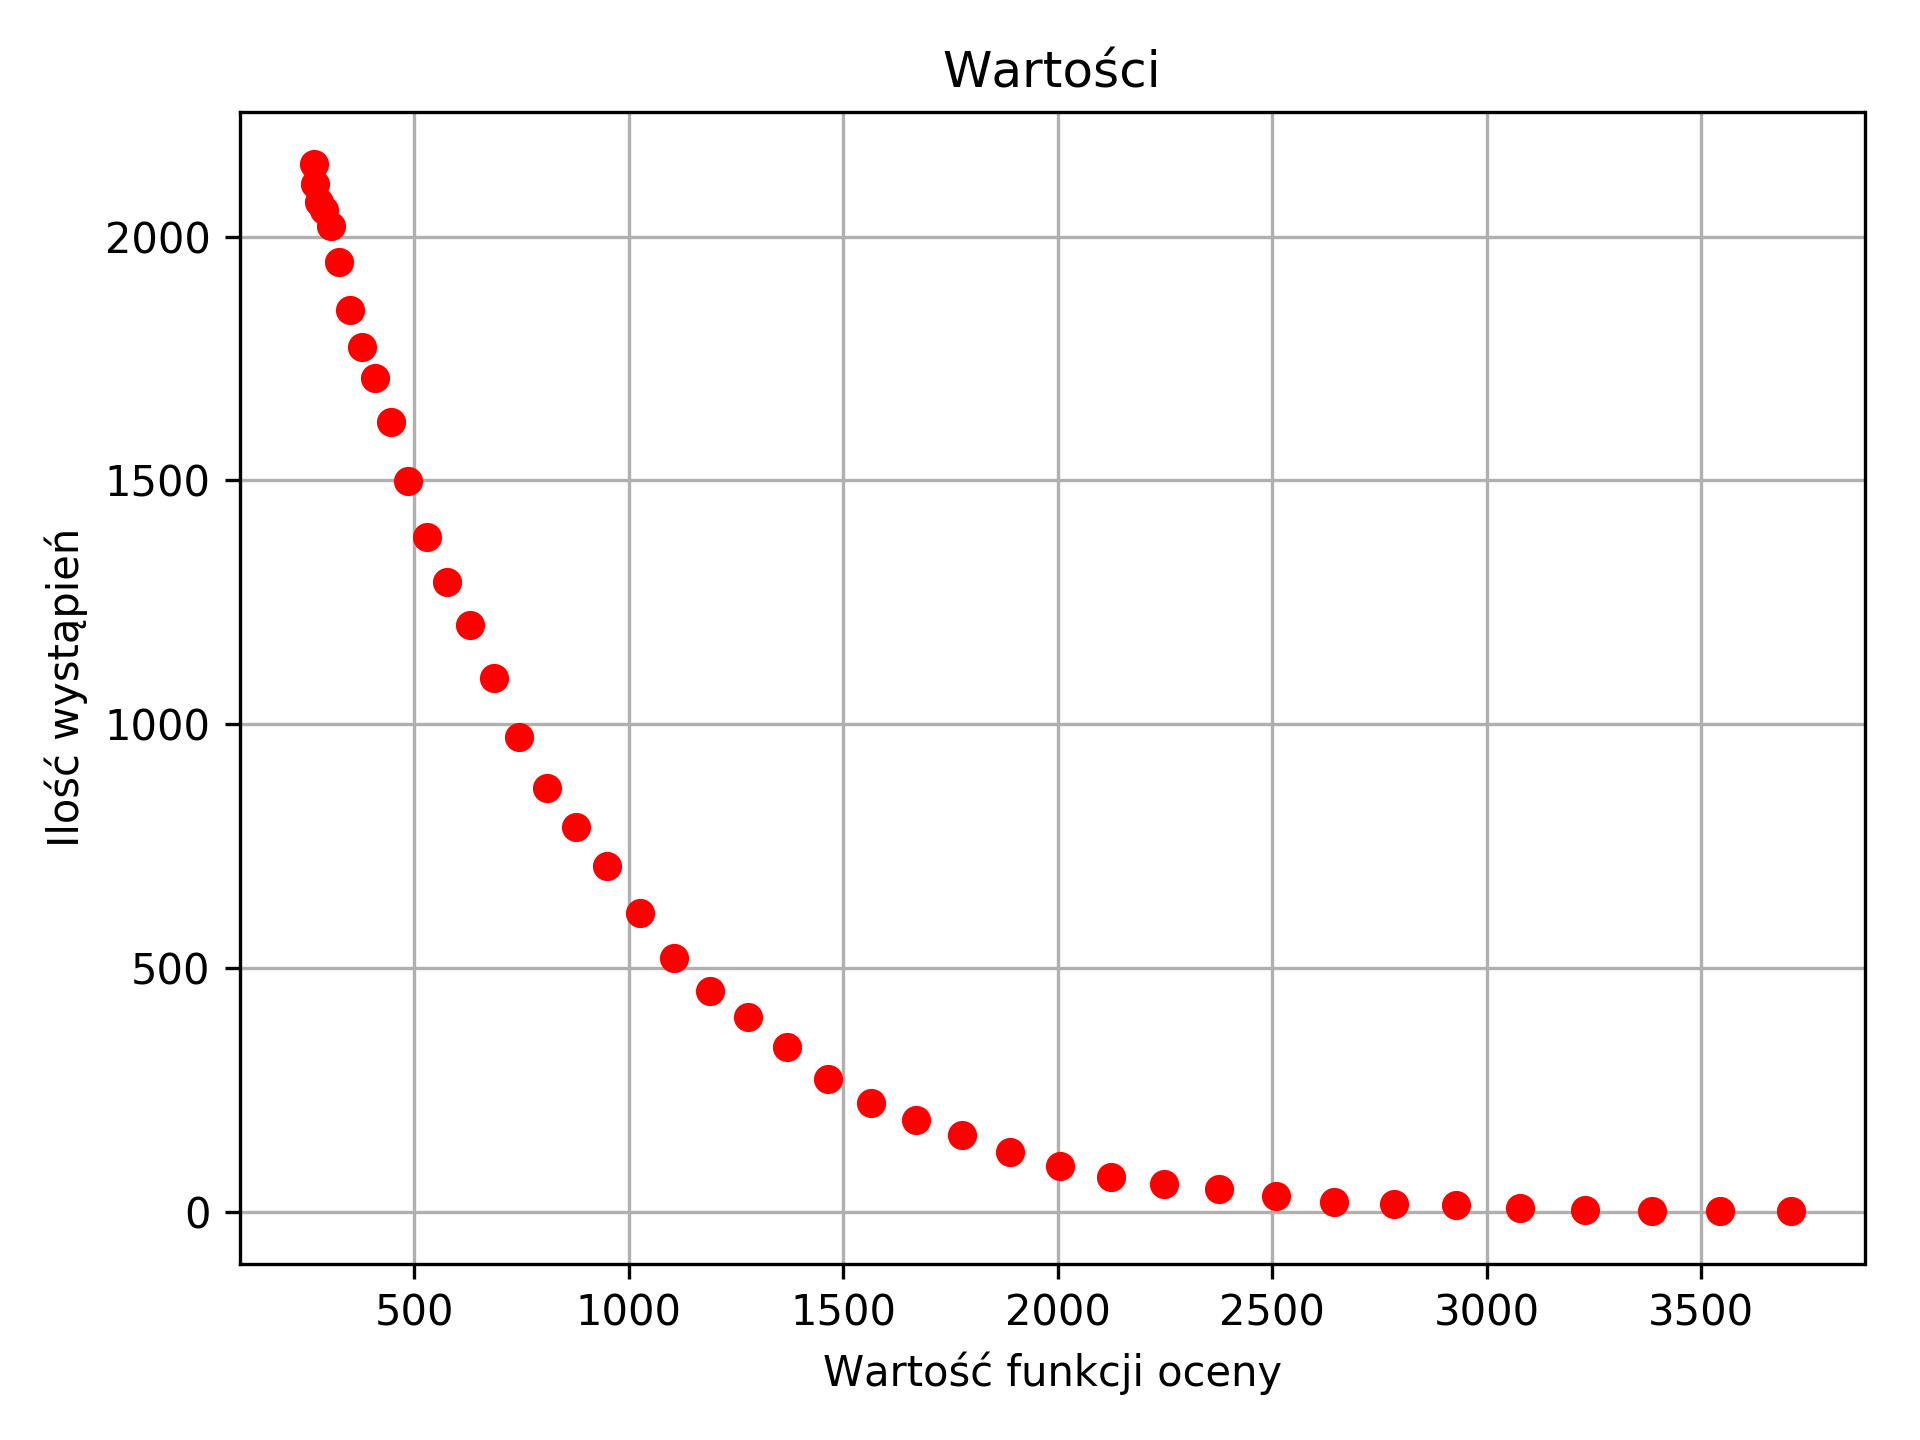
\includegraphics[width=0.55\textwidth]{1Values.png}
	\caption{Ilość kart równa 15, wartość na pierwszym stosie 25, a na drugim 30. Wartości kart: 8, 3, 4, 4, 10, 1, 8, 4, 2, 6, 9, 10, 1, 4, 4.}
	\label{fig1}
\end{figure}

\newpage

\begin{figure}[h]
	\centering					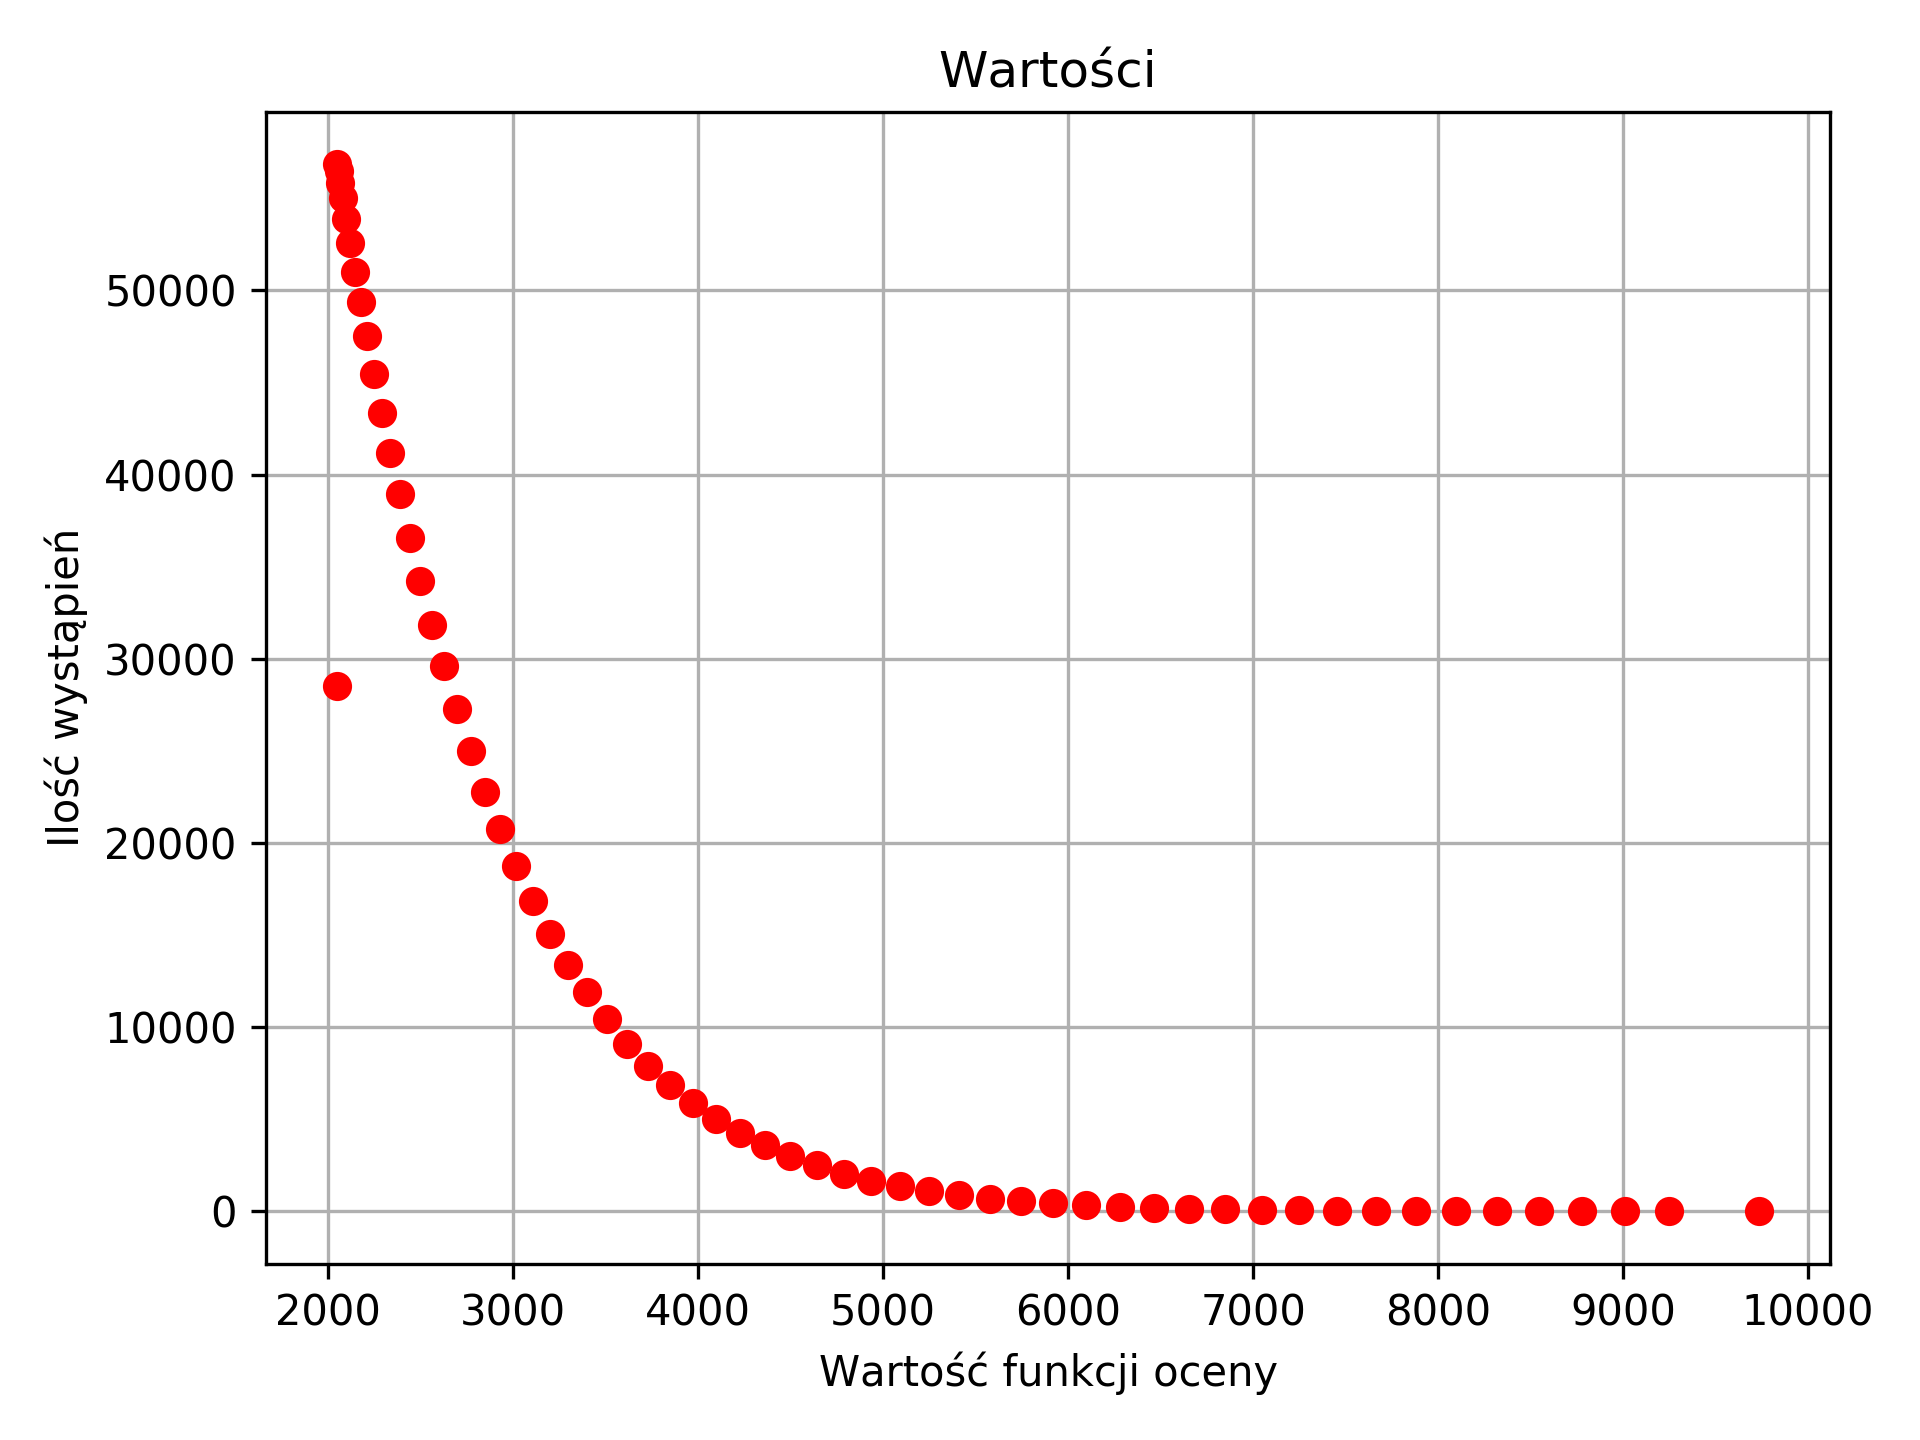
\includegraphics[width=0.55\textwidth]{2Values.png}
	\caption{Ilość kart równa 20, wartość na pierwszym stosie 25, a na drugim 30. Wartości kart: 4, 4, 10, 9, 8, 8, 9, 4, 4, 5, 8, 7, 5, 5, 4, 3, 6, 6, 2, 8.}
	\label{fig1}
\end{figure}

Jak widać, wraz ze zmniejszaniem się wartości funkcji celu zwiększa się liczba wystąpień danej oceny. Co ciekawe w przypadku ukazanym na rysunku nr. 13 możliwych do uzyskania było tylko 42 różnych wartości funkcji celu, a w przypadku drugim 62. Są to liczby niespodziewanie małe, lecz wynikają one z wartości kart i sposobu oceny.  

Jak można zauważyć, rozwiązanie optymalne lub bliskie optymalnego stanowią lwią część wszystkich wartości i stanowią w zależności od przyjęcia górnej granicy nawet do 30\% wszystkich możliwości, stąd dla populacji o liczności równej np. 10 nie sposób by nie została wylosowana jedna z takich wartości.

Zupełnie inaczej przedstawia się przestrzeń przy zadaniu, w którym wartości kart na stosach są zupełnie różne. Aby to pokazać, przeanalizowano przestrzeń dwudzestokartową w której na pierwszym stosie oczekujemy wartości 110, na drugim zaś 0. Wyniki zaprezentowano na poniższym histogramie:
\begin{figure}[H]
	\centering					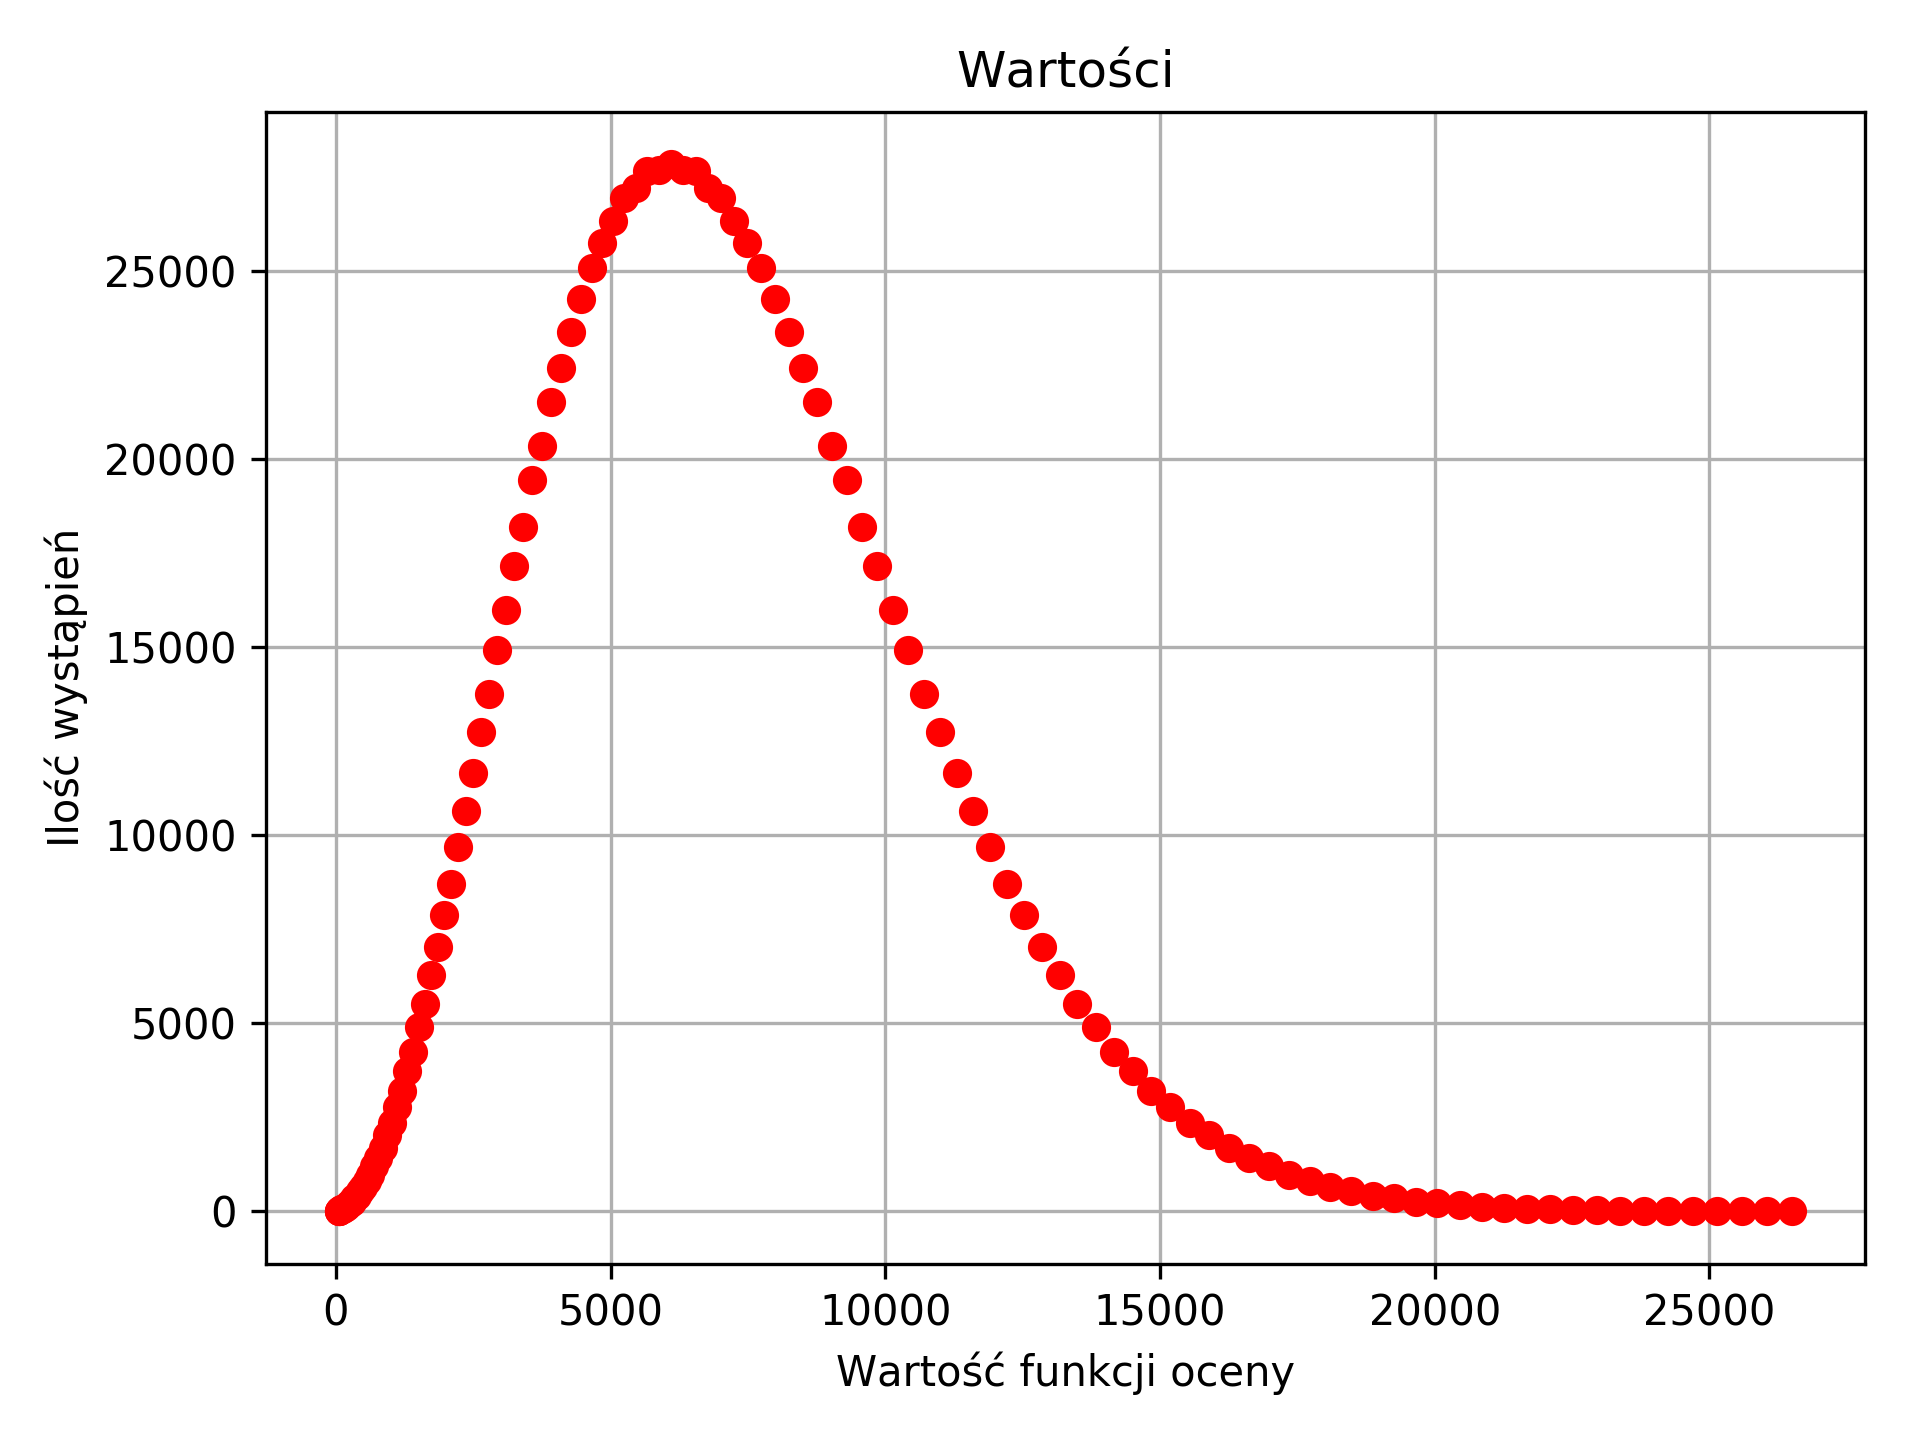
\includegraphics[width=0.55\textwidth]{3Values.png}
	\caption{Ilość kart równa 20, wartość na pierwszym stosie 110, a na drugim 0. Wartości kart losowe.}
	\label{fig1}
\end{figure}

W tej "trudnej" przestrzeni wykresy przedstawiające zbieganie się wartości minimalnej w iteracji przedstawiają się ciekawiej:
\begin{figure}[H]
	\centering					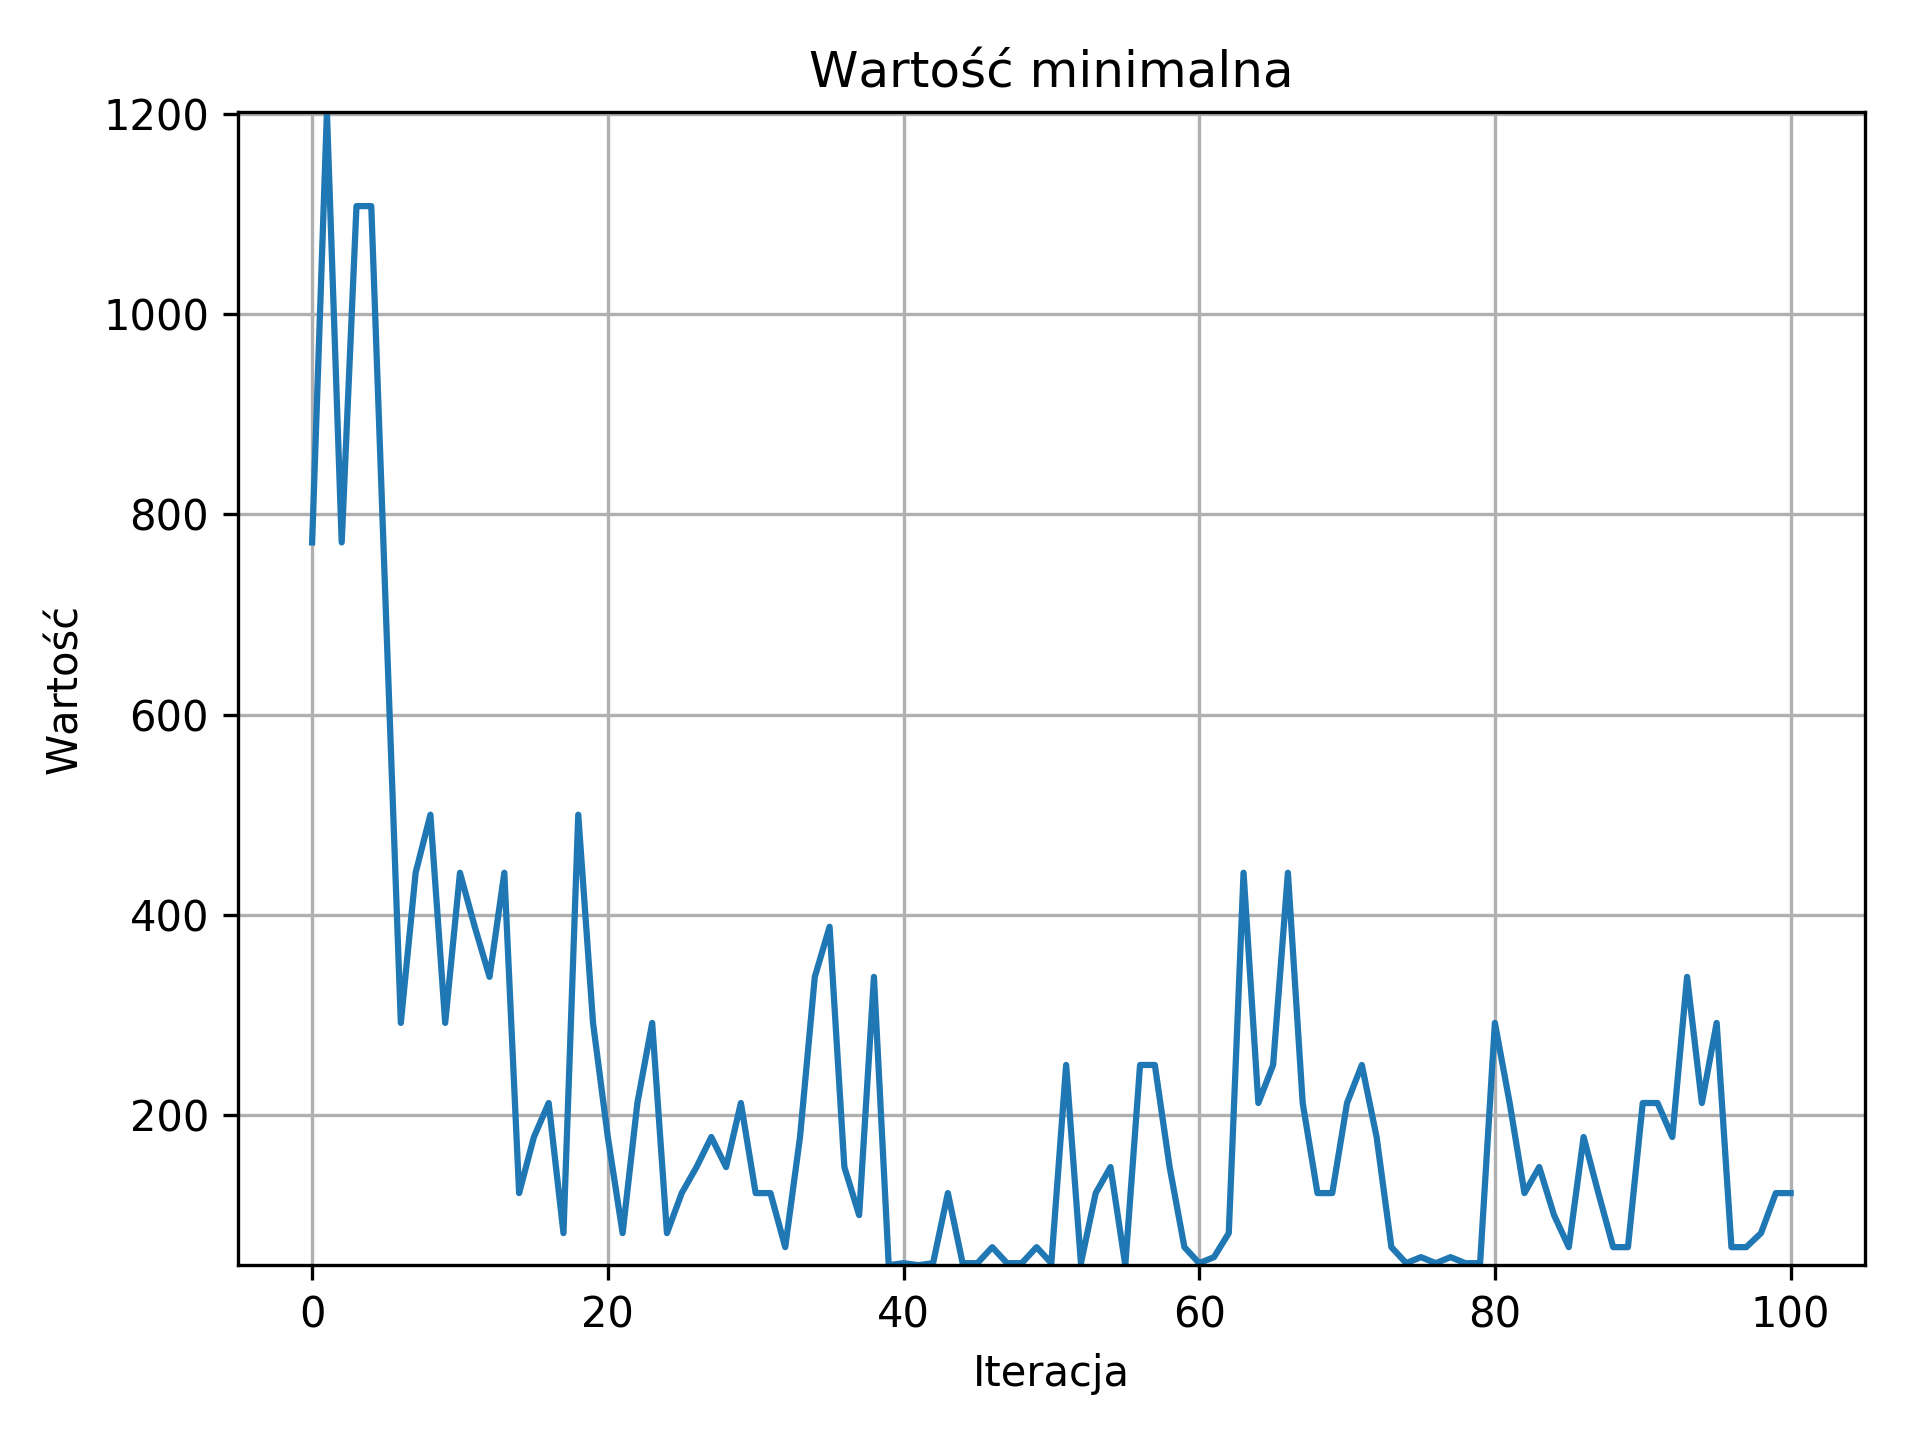
\includegraphics[width=0.55\textwidth]{one_group.png}
	\caption{Minimlna wartość funkcji celu w zależności od numeru iteracji, problem "trudny".}
	\label{fig1}
\end{figure}
W tym przypadku widać, że początkowa populacja nie zawiera dobrych rozwiązań. Dopiero po około 40 iteracjach udaje się znaleźć rozwiązanie bliskie optymalnemu. Dzieje się tak dlatego, że dobrych rozwiązań jest w tej przestrzeni znacznie mniej, niż w przestrzeni "łatwej", a co za tym idzie "trafienie" do optimum przy pomocy krzyżowania i mutacji jest znacznie mniej prawdopodobne.

\section{Podsumowanie}
Do rozwiązanie problemu został zaimplementowany poprawny algorytm ewolucyjny z wieloma możliwościami parametryzacji. Przy wybranej funkcji celu i zadanej przestrzeni nie można poprawnie zobrazować działania algorytmu przy znajdowaniu najmniejszej wartości. Sytuacja mogłaby ulec zmianie w przypadku dodania dodatkowych celów do spełnienia np. podobnej ilości kart lub jak najmniejszego odchylenia standardowego ich wartości.  
 
\end{document}
